% A LaTeX template for MSc Project submissions to 
% Politecnico di Milano (PoliMi) - School of Industrial and Information Engineering
%
% S. Bonetti, A. Gruttadauria, G. Mescolini, A. Zingaro
% e-mail: template-tesi-ingind@polimi.it
%
% Last Revision: October 2021
%
% Copyright 2021 Politecnico di Milano, Italy. NC-BY

\documentclass{Configuration_Files/PoliMi3i_project}

%------------------------------------------------------------------------------
%	REQUIRED PACKAGES AND  CONFIGURATIONS
%------------------------------------------------------------------------------

% CONFIGURATIONS
\usepackage{parskip} % For paragraph layout
\usepackage{setspace} % For using single or double spacing
\usepackage{emptypage} % To insert empty pages
\usepackage{multicol} % To write in multiple columns (executive summary)
\setlength\columnsep{15pt} % Column separation in executive summary
\setlength\parindent{10pt} % Indentation
\raggedbottom  

% PACKAGES FOR TITLES
\usepackage{titlesec}
% \titlespacing{\section}{left spacing}{before spacing}{after spacing}
\titlespacing{\section}{0pt}{3.3ex}{2ex}
\titlespacing{\subsection}{0pt}{3.3ex}{1.65ex}
\titlespacing{\subsubsection}{0pt}{3.3ex}{1ex}
\usepackage{color}

% PACKAGES FOR LANGUAGE AND FONT
\usepackage[english]{babel} % The document is in English  
\usepackage[utf8]{inputenc} % UTF8 encoding
\usepackage[T1]{fontenc} % Font encoding
\usepackage[11pt]{moresize} % Big fonts

% PACKAGES FOR IMAGES
\usepackage{graphicx}
\usepackage{svg}
\usepackage{transparent} % Enables transparent images
\usepackage{eso-pic} % For the background picture on the title page
%\usepackage{subfig} % Numbered and caption subfigures using \subfloat.
\usepackage[export]{adjustbox}
\usepackage{tikz} % A package for high-quality hand-made figures.
\usetikzlibrary{}
\graphicspath{{./Images/}} % Directory of the images
\usepackage{caption} % Coloured captions
\usepackage{subcaption}
\usepackage{xcolor} % Coloured captions
\usepackage{amsthm,thmtools,xcolor} % Coloured "Theorem"
\usepackage{float}

% STANDARD MATH PACKAGES
\usepackage{amsmath}
\usepackage{amsthm}
\usepackage{amssymb}
\usepackage{amsfonts}
\usepackage{bm}
\usepackage{cancel}
\usepackage[overload]{empheq} % For braced-style systems of equations.
\usepackage{fix-cm} % To override original LaTeX restrictions on sizes

% PACKAGES FOR TABLES
\usepackage{tabularx}
\usepackage{longtable} % Tables that can span several pages
\usepackage{colortbl}

% PACKAGES FOR ALGORITHMS (PSEUDO-CODE)
\usepackage{algorithm}
\usepackage{algorithmic}

% PACKAGES FOR REFERENCES & BIBLIOGRAPHY
\usepackage[colorlinks=true,linkcolor=black,anchorcolor=black,citecolor=black,filecolor=black,menucolor=black,runcolor=black,urlcolor=black]{hyperref} % Adds clickable links at references
\usepackage{cleveref}
\usepackage[square, numbers, sort&compress]{natbib} % Square brackets, citing references with numbers, citations sorted by appearance in the text and compressed
\bibliographystyle{abbrvnat} % You may use a different style adapted to your field

% OTHER PACKAGES
\usepackage{pdfpages} % To include a pdf file
\usepackage{afterpage}
\usepackage{lipsum} % DUMMY PACKAGE
\usepackage{fancyhdr} % For the headers
\usepackage{fancyvrb}
\usepackage[acronym]{glossaries}
\usepackage{enumitem} 

\usepackage{listings}
\usepackage{alloy-style}
\fancyhf{}

% Input of configuration file. Do not change config.tex file unless you really know what you are doing. 
% Define blue color typical of polimi
\definecolor{bluepoli}{cmyk}{0.4,0.1,0,0.4}
\definecolor{Green}{RGB}{30, 170, 0}

% Custom theorem environments
\declaretheoremstyle[
  headfont=\color{bluepoli}\normalfont\bfseries,
  bodyfont=\color{black}\normalfont\itshape,
]{colored}

% Set-up caption colors
%\captionsetup[figure]{labelfont={color=bluepoli}} % Set colour of the captions
%\captionsetup[table]{labelfont={color=bluepoli}} % Set colour of the captions
%\captionsetup[algorithm]{labelfont={color=bluepoli}} % Set colour of the captions
\captionsetup{font=bf}

\theoremstyle{colored}
\newtheorem{theorem}{Theorem}[chapter]
\newtheorem{proposition}{Proposition}[chapter]
\newtheorem{definition}{Definition}[chapter]

% Enhances the features of the standard "table" and "tabular" environments.
\newcommand\T{\rule{0pt}{2.6ex}}
\newcommand\B{\rule[-1.2ex]{0pt}{0pt}}

% Pseudo-code algorithm descriptions.
\newcounter{algsubstate}
\renewcommand{\thealgsubstate}{\alph{algsubstate}}
\newenvironment{algsubstates}
  {\setcounter{algsubstate}{0}%
   \renewcommand{\STATE}{%
     \stepcounter{algsubstate}%
     \Statex {\small\thealgsubstate:}\space}}
  {}

% New font size
\newcommand\numfontsize{\@setfontsize\Huge{200}{60}}

% Title format: chapter
\titleformat{\chapter}[hang]{
\fontsize{50}{20}\selectfont\bfseries\filright}{\textcolor{bluepoli} \thechapter\hsp\hspace{2mm}\textcolor{bluepoli}{|   }\hsp}{0pt}{\huge\bfseries \textcolor{bluepoli}
}

% Title format: section
\titleformat{\section}
{\normalfont\Large\bfseries}
{\thesection.}{1em}{}
%{\color{bluepoli}\normalfont\Large\bfseries}
%{\color{bluepoli}\thesection.}{1em}{}

% Title format: subsection
\titleformat{\subsection}
{\normalfont\large\bfseries}
{\thesubsection.}{1em}{}
%{\color{bluepoli}\normalfont\large\bfseries}
%{\color{bluepoli}\thesubsection.}{1em}{}

% Title format: subsubsection
\titleformat{\subsubsection}
{\normalfont\bfseries}
{\thesubsubsection.}{1em}{}
%{\color{bluepoli}\normalfont\large\bfseries}
%{\color{bluepoli}\thesubsubsection.}{1em}{}

% Shortening for setting no horizontal-spacing
\newcommand{\hsp}{\hspace{0pt}}

\makeatletter
% Renewcommand: cleardoublepage including the background pic
\renewcommand*\cleardoublepage{%
  \clearpage
}
\makeatother

%For correctly numbering algorithms
\numberwithin{algorithm}{chapter}

%----------------------------------------------------------------------------
%	NEW COMMANDS DEFINED
%----------------------------------------------------------------------------

% EXAMPLES OF NEW COMMANDS
\newcommand{\bea}{\begin{eqnarray}} % Shortcut for equation arrays
\newcommand{\eea}{\end{eqnarray}}
\newcommand{\e}[1]{\times 10^{#1}}  % Powers of 10 notation

%----------------------------------------------------------------------------
%	ADD YOUR PACKAGES (be careful of package interaction)
%----------------------------------------------------------------------------

%----------------------------------------------------------------------------
%	ADD YOUR DEFINITIONS AND COMMANDS (be careful of existing commands)
%----------------------------------------------------------------------------


% Common abbrev. are set as commands to ensure proper spacing after the dot
\RequirePackage{xspace}
\newcommand{\ie}{i.e.\@\xspace}
\newcommand{\aka}{a.k.a.\@\xspace}
\newcommand{\Ie}{I.e.\@\xspace}
\newcommand{\cf}{cf.\@\xspace}
\newcommand{\Cf}{Cf.\@\xspace}
\newcommand{\eg}{e.g.\@\xspace}
\newcommand{\Eg}{E.g.\@\xspace}
\newcommand{\etal}{et al.\@\xspace}
\newcommand{\etc}{etc.\@\xspace}
\newcommand{\wrt}{w.r.t.\@\xspace}
\newcommand{\Wrt}{W.r.t.\@\xspace}
% TODO: Remove on final doc
\RequirePackage[textsize=scriptsize,color=blue!20]{todonotes}
\newcounter{comment}
\newcommand{\comment}[2][]{%
% initials of the author (optional) + note in the margin
\refstepcounter{comment}%
{%
\todo{\textbf{Comment [#1\thecomment]:}~#2}%
}}
% END TODO

\usepackage{soul}
\usepackage{tikz}

\usetikzlibrary{calc}
\usetikzlibrary{decorations.pathmorphing}


\makeatletter

\newcommand{\defhighlighter}[3][]{%
  \tikzset{every highlighter/.style={color=#2, fill opacity=#3, #1}}%
}

\defhighlighter{yellow}{.5}

\newcommand{\highlight@DoHighlight}{
  \fill [ decoration = {random steps, amplitude=1pt, segment length=15pt}
        , outer sep = -15pt, inner sep = 0pt, decorate
       , every highlighter, this highlighter ]
        ($(begin highlight)+(0,8pt)$) rectangle ($(end highlight)+(0,-3pt)$) ;
}

\newcommand{\highlight@BeginHighlight}{
  \coordinate (begin highlight) at (0,0) ;
}

\newcommand{\highlight@EndHighlight}{
  \coordinate (end highlight) at (0,0) ;
}

\newdimen\highlight@previous
\newdimen\highlight@current

\DeclareRobustCommand*\highlight[1][]{%
  \tikzset{this highlighter/.style={#1}}%
  \SOUL@setup
  %
  \def\SOUL@preamble{%
    \begin{tikzpicture}[overlay, remember picture]
      \highlight@BeginHighlight
      \highlight@EndHighlight
    \end{tikzpicture}%
  }%
  %
  \def\SOUL@postamble{%
    \begin{tikzpicture}[overlay, remember picture]
      \highlight@EndHighlight
      \highlight@DoHighlight
    \end{tikzpicture}%
  }%
  %
  \def\SOUL@everyhyphen{%
    \discretionary{%
      \SOUL@setkern\SOUL@hyphkern
      \SOUL@sethyphenchar
      \tikz[overlay, remember picture] \highlight@EndHighlight ;%
    }{%
    }{%
      \SOUL@setkern\SOUL@charkern
    }%
  }%
  %
  \def\SOUL@everyexhyphen##1{%
    \SOUL@setkern\SOUL@hyphkern
    \hbox{##1}%
    \discretionary{%
      \tikz[overlay, remember picture] \highlight@EndHighlight ;%
    }{%
    }{%
      \SOUL@setkern\SOUL@charkern
    }%
  }%
  %
  \def\SOUL@everysyllable{%
    \begin{tikzpicture}[overlay, remember picture]
      \path let \p0 = (begin highlight), \p1 = (0,0) in \pgfextra
        \global\highlight@previous=\y0
        \global\highlight@current =\y1
      \endpgfextra (0,0) ;
      \ifdim\highlight@current < \highlight@previous
        \highlight@DoHighlight
        \highlight@BeginHighlight
      \fi
    \end{tikzpicture}%
    \the\SOUL@syllable
    \tikz[overlay, remember picture] \highlight@EndHighlight ;%
  }%
  \SOUL@
}

\makeatother

\makeglossaries

\newacronym{acronym}{ACR}{Acronym}

%----------------------------------------------------------------------------
%	BEGIN OF YOUR DOCUMENT
%----------------------------------------------------------------------------

\begin{document}

\fancypagestyle{plain}{%
\fancyhf{} % Clear all header and footer fields
\fancyhead[RO,RE]{\thepage} %RO=right odd, RE=right even
\renewcommand{\headrulewidth}{0pt}
\renewcommand{\footrulewidth}{0pt}}


%----------------------------------------------------------------------------
%	TITLE PAGE
%----------------------------------------------------------------------------

\pagestyle{empty} % No page numbers
\frontmatter % Use roman page numbering style (i, ii, iii, iv...) for the preamble pages

\puttitle{
	title= Requirement Analysis and Specification Document\\ \emph{Code Kata Battle}, % Title of the project
	name= Andaloro Emanuele & 10692544 \\ 
  Galantino Claudia & & & 11011392 \\
  Lew Deveali Simon & & 10986407,% Author Name and Surname
	course=Software engineering II
 \\Computer Science and Engineering \\, % Study Programme (in Italian)
	ID  =  11,  % Student ID number (numero di matricola)
 advisor={},
	coadvisor={}, % Co-Supervisor name, remove this line if there is none
	academicyear={2023-24},% Academic Year
 }
%----------------------------------------------------------------------------
%	PREAMBLE PAGES: ABSTRACT (inglese e italiano), EXECUTIVE SUMMARY
%----------------------------------------------------------------------------

%	LIST OF CONTENTS/FIGURES/TABLES/SYMBOLS
%----------------------------------------------------------------------------

% TABLE OF CONTENTS\thispagestyle{empty}
\tableofcontents % Table of contents 
\thispagestyle{empty}


%-------------------------------------------------------------------------
%	THESIS MAIN TEXT
%-------------------------------------------------------------------------
% In the main text of your project you can write the chapters in two different ways:
%
%(1) As presented in this template you can write:
%    \chapter{Title of the chapter}
%    *body of the chapter*
%
%(2) You can write your chapter in a separated .tex file and then include it in the main file with the following command:
%    \chapter{Title of the chapter}
%    \input{chapter_file.tex}
%
% Especially for long project, we recommend you the second option.

\addtocontents{toc}{\vspace{2em}} % Add a gap in the Contents, for aesthetics
\mainmatter % Begin numeric (1,2,3...) page numbering

% --------------------------------------------------------------------------
% NUMBERED CHAPTERS % Regular chapters following
% --------------------------------------------------------------------------
%------------------------------------------------------------------------------------------------------------------------------------------------
\clearpage
{{\chapter{Introduction}}}
\label{sect:introduction}
\section{Purpose}
As the software industry grows, training better developers is becoming more and more important. Traditionally, developers are trained solely in theory and then thrust into working on a whole complex project without any previous practice. That is what code katas try to tackle. Code katas are short exercises that can be completed in minutes. Some involve programming while others involve thinking about the issues behind programming. In general, code katas are unlikely to have a single correct answer, but the main point of the kata is what you learn along the way.
CodeKataBattle (CKB) is a new platform where Educators can create tournaments comprising multiple battles. Each battle consists of one particular code kata and aims to develop several skills. The idea is that students compete in these tournaments in teams to gain hands-on experience and improve their software development skills. The main goals of the platform are the following:

\subsection{Goals}
\begin{enumerate}[label={[G\arabic*]}]
    \item Educators create code kata battles 
    \item Students compete in multiple tournaments in teams
    \item Students receive performance feedback after each battle assessment%Students are assessed and receive feedback about their performance in each battle
\end{enumerate}

\section{Scope}
In this section, we will try to identify CKB plataform domain. 
There are to main users that interact with the system: Educators and students.

Educators are the one who create the tournaments which consist of several battles grouped by context. For each battle, they will have to provide not only the code kata, but also the number of allowed participants and a deadline for both registration and submission. Another important feature is that they can allow other colleagues to add new battles to the tournament. In addition, to make the tournament a competition, they have to establish the scoring criteria.
Lastly, for each tournament Educators will create badges which will be assigned to each students who fulfill some specific rule indicated into the badge itself.

Students will be able to enrol in one of these tournaments in groups. Later, the platform will notify them when the competition starts and provide them with the repository with all the code necessary for the kata. Students have to fork this repository and then can start working in the solution. They will also have to set a Github action\footnote{We use the term action to match the assigment however we think that it should be WebHook} so every push they commit to the repository during the competition is accounted for the computation of their score. Finally, after the deadline, the systems elaborate a rank considering their best score and the manual evaluation performed by the educator.
\subsection{World Phenomena}


\begin{enumerate}[label={[WP\arabic*]}]
    \item Educators think of a new kata, code the automation  scripts and crate a test suite for the battle
    \item Students create a Github account
    \item Students fork the repository of the code kata provided

    \item Students code the kata in their preferred IDE and commit to their repository
    \item Educators think of a proper criteria to evaluate students work
\end{enumerate}
\subsection{Shared Phenomena}
 \textbf{World controlled}
\begin{enumerate}[label={[SP\arabic*]}]
    \item Students set up an automated workflow through github actions
    \item Educators create tournaments, battles and badges. 
    \item Students invite others to join their team
    \item A member of the team register his team to participate in a tournament
    \item GitHub informs the CKB platform about new pushes in the students repository
    \item Educators assign their personal evaluation once the submission deadline expires
    
 \textbf{Machine controlled}

  \item The system creates a GitHub repository and sends the link to the students belonging to teams enroled in a specific battle after the registration deadline.
  \item The system updates the score evaluation as soon a new push is performed
  \item The system assigns a badge to the students who satisfies the predefined rules and the students are able to see it
\end{enumerate}

\section{Definitions, Acronyms, Abbreviations}
\subsection{Definitions}
\begin{enumerate} [label=\textbullet]
    \item \textbf{Static analysis tool} :Method of debugging that is done by automatically examining the source code without having to execute the program ensuring that is  compliant, safe, and secure.
    \item \textbf{Dynamic analysis tool} :Process of testing and evaluating a programme thanks to running a test on the code.
    \item \textbf{OAuth Access Token} :An OAuth Access Token is a string that the OAuth client uses to make requests to the resource server.
    \item \textbf{WebHook} :A webhook is an HTTP-based callback function that allows lightweight, event-driven communication between 2 application programming interfaces (APIs). In this case it lets communication between Code Kata Battle platform and GitHub.
    \item \textbf{Consolidation} : Is a phase that occurs at the end of a tournament where the educator can decide to add a manual evaluation.
\end{enumerate}
\subsection{Acronyms}
    \begin{enumerate}[label=\textbullet]
        \item CKB: Code kata battle;
        \item UI: User Interface;
        \item UML: Unified Modelling Language.
    \end{enumerate}

\subsection{Abbreviations}
\begin{enumerate}[label=\textbullet]
    \item G*: goal
    \item WP*: world phenomena
    \item SP*: shared phenomena
    \item R*: functional requirement
    \item UC*: use case
\end{enumerate}
    
\section{Revision history}
        \begin{enumerate}[label=\textbullet]
            \item Version 1.0 (20/12/2023)
        \end{enumerate}
\pagebreak
\section{Reference Documents}
The document is based on the following materials:
    \begin{enumerate}[label=\textbullet]
        \item The specification of the RASD and DD assignment of the Software Engineering II course a.a. 2023/24
        \item Slides of the course on WeBeep
    \end{enumerate}

\section{Document Structure}

    \begin{enumerate}[label=\arabic*., align=left]
        \item \textbf{Introduction: }it aims to give a brief description of the project. In particular it’s focused on the reasons and the goals that are going to be achieved with its development;
        \item \textbf{Overall Description: }it is an high-level description of how the system works with a detailed explanation of the phenomena that involve the world,the machine or both,there is also the domain description with its assumptions;
        \item \textbf{Specific Requirements: }in this section there is a detailed  analysis of the requirements needed to achieve the goals.Moreover, it contains more information useful for developers (i.e constraints about HW and SW);
        \item \textbf{Formal analysis: }it's a formal description of the world phenomena by the means of Alloy;
        \item \textbf{Effort spent: }it shows the time spent to realize this document organized by section;
         \item \textbf{References: }it contains the references to any documents and software used to write this paper.
        
    \end{enumerate}


%------------------------------------------------------------------------------------------------------------------------------------------------
\clearpage
{{\chapter{Overall Description}}}
\label{sect:overview}
\section{Product perspective}
\subsection{Scenarios}

\subsubsection{ Educator creates a tournament }
The educator A wants to create a new tournament, he enters the KCB with his educator credentials, once on the homepage he can go into the section "create a new tournament" and fill out a form asking name, main context, enrolment deadline. Now he is able to create or add battles for it.

\subsubsection{ Educator creates a Battle for a specific tournament}
The educator B, owner of a tournament 1, wants to create a battle for his tournament. He enters the KCB with his educator credentials, he goes into the tournament section, selects the tournament 1, and he can go into the "create new battle" section. In this section he can fill a form with the data of the battle such as the battle name, the code template, the registration deadline, the final submission deadline, the quality aspects of that battle which are used for the scoring and sets the minimum and the maximum number of students per group that can participate in that battle. The educator defines a set of categories such that :

    -functional aspects: measured in terms of the number of test cases that pass out of all test cases; 
    
    -timeliness, measured in terms of the time passed between the registration deadline and the last commit;
    
    -quality level:extracted through static analysis tools that consider multiple aspects such as reliability, security, and so on.

The educator gives to each category a  weight.    

\subsubsection{Owner gives permission to another educator to add a Battle}
The owner, the educator C, goes to the section dedicated to the tournament and gives permission to other educators to create new battles by pressing a button to share the control of a tournament. As a consequence the system shows the educator a bar that let him to search other educators. The educator can choose the other educators so an educator D can create a new battle, filling the same form described in the previous scenario. 

\subsubsection{ A student creates a team and invites others to join}
Student E, who already has a profile on the platform, will receive a notification as soon as a new tournament is created. Once he is on the platform, he can read the main information about the tournament and decide whether to join it by the given deadline.
He can create a team for a battle inviting other students, respecting the minimum number of student imposed for the battle of that tournament. To do that, the student will share with his teammate a link to join the battle.

\subsubsection{ A member of the team enrols in a battle}
Student F wants to join her friend on a team for a battle, she received an email with the link that allows her to participate in the battle. She opens the link and thanks to her platform credentials she can join his friend's team.
She knows that students cannot join more than one team for a specific battle.
Once on the platform, she will be able to see in the tournament section the tournament she has registered in and the team she just joined.

\subsubsection{The battle begins}
As soon as the deadline expires, the platform creates the GitHub repository and for each team enrolled sends a notification with a link containing the code kata of the battle. The student G, who has enrolled into this battle, after receiving the notification opens the link and use his credentials to access the source code provided.

\subsubsection{A member of the team pushes and commit to the kata repository}
Student H who is enrolled in a battle, finishes to code the kata with his teammates and wants to submit it. In order to do that, he should fork the GitHub repository of the kata and set up the automated workflow if no one has done it before.
Thanks to this action the platform will be triggered every time any of the team members pushes a new commit into the main branch of the repository. Afterwards he pushes and commits being able to see the new results on the platform.

\subsubsection{ The battle ends}
At the end of the battle the platform updates the tournament score of every student enrolled, by recomputing the scores considering all battles belonging to that tournament.


\subsubsection{ Educator manually evaluates the code provided by students}
Educator L who contributed to the creation of the tournament has the possibility to manually evaluate the work done by a team at the end of each battle. In order to do that, he can access the platform with his credentials, and go to the tournament section, then open the battle information and go through the sources produced by each team. Afterwards, he will assign a score that will be considered by the platform when the final ranking is computed.

\subsubsection{ Users see the final rank of the tournament}
Educator M closes the tournament thanks to the button 'end tournament' in the tournament section of the KCB platform. As a consequence of that, the platform elaborate the final rank for each student involved to that tournament and finally notify them about it. 
Student N who participated to the tournament and received the notification via e-mail can consult the final ranking by selecting the tournament into the 'tournament section' of the platform.

\subsubsection{ Users can see current rank}
User J (an educators or a student) involved in a battle is allowed to see the evolving rank during the battles. They can consult the ranking into the dedicated section of the battle and compare students' performances.
Every user has the possibility to consult the "ongoing tournament section"in which it is possible to see the list of the ranking for each tournament in progress. 

\subsubsection{Student receives a badge}
When a tournament ends the platform assign the badges to the students that satisfied the requirements to obtain them.
As previously mentioned, the criteria for assigning the badge are defined by the educators during the creation of the tournament.
Any user subscribed to the platform can view the badges collected by any student so far. So student P who want to see the total number of badges can access the platform with his credentials and see them on his profile. He can also view the badges collected by his friend Student Q, in order to do that he can look for student Q profile and check the number of badges his friend has collected so far.
\pagebreak



\subsection{ Domain class diagram}
\begin{figure}[h!]
\centering
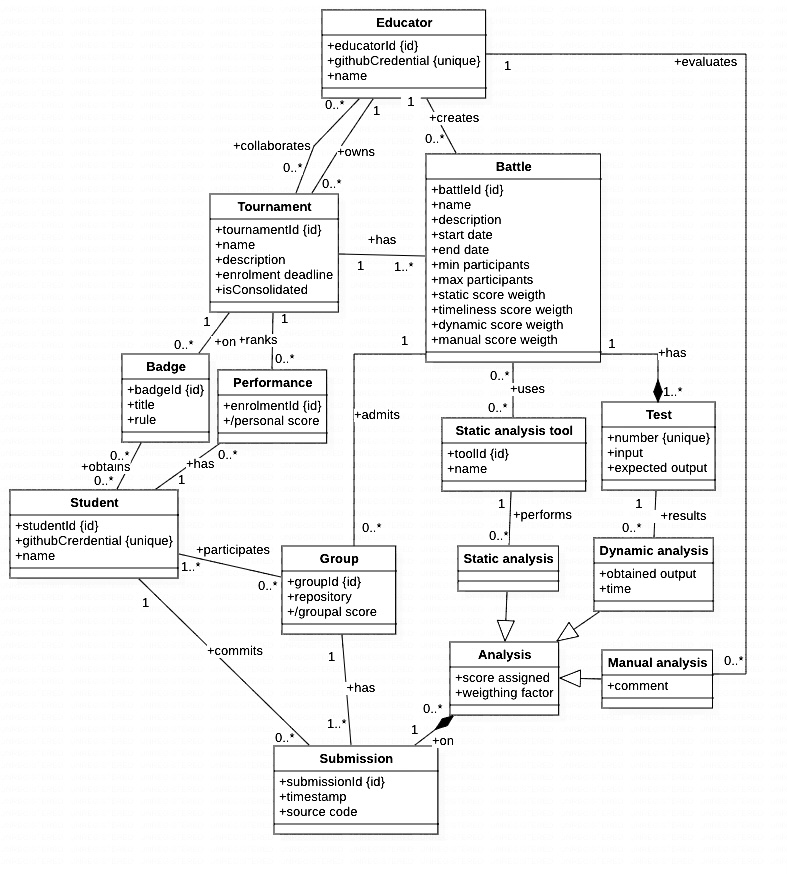
\includegraphics[width=\textwidth]{Images/dcd.jpg}
\caption{Domain class diagram}
\label{dcd}
\end{figure}

In Figure \labelcref{dcd} you can find the domain class diagram. Despite both educators and students being user, we represent  them separately in the diagram.  As it was mentioned educators can own a tournament or simply collaborate in other's. The tournament has only one owner but can have many collaborators. 

Tournaments consists of many battles which are created for that specific tournament. Then for the scoring it is necessary that the battle has the weights for each type of analysis (static, timeliness, dynamic and manual). As well as the static tools to be used and the tests to evaluate that specific battle.

Afterwards, with all this different types of analysis it will be possible to perform the whole analysis on a particular submission. All the analysis regardless of the type will contribute on the score of the submission similarly. Note that Timeliness is not represented like the other analysis because the submission already contains the timestamp which is sufficient for that purpose. Although it could not be represented in the diagram, the weighing factor of the analysis, the tools used and the executed tests have to be consistent with the ones defined in the battle that submission corresponds. In the same way, the educator who evaluates should be the one responsible of that battle.

In order to participate in a battle students have to make a group this is only correspond to one battle and contains the Github repository from which submissions will be collected each time the source code is modified and committed. Then the score of the group will be taken from the best submission. In the diagram we could not represent that students can only participate only once in a battle, however this is relevant.

Finally, the tournament will have many badges which then will be assigned to the students following the rule criteria. This was not represented neither that students can only have badges for tournaments in which the took part.

\subsection{State diagrams}
In this subsection there is a discussion of the state charts diagram the ones for the management of the battles and the tournaments.Both of them are necessary for having a better understanding of how battles and tournaments works.

\textbf{Tournament management}

\begin{figure}[h!]
\centering
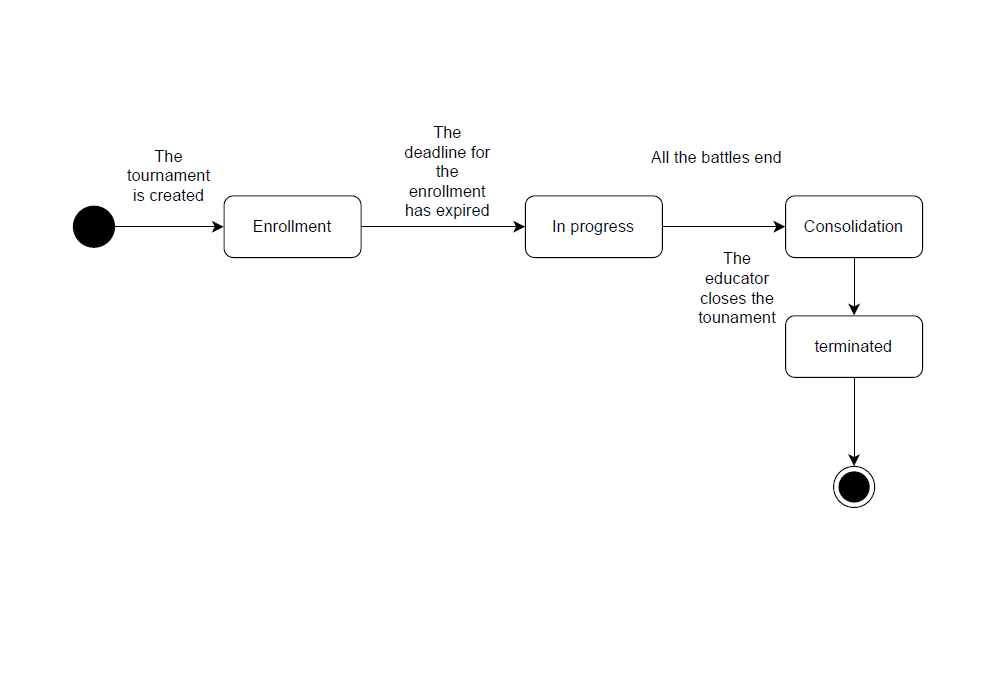
\includegraphics[width=12cm]{Images/tournament.png}
\caption{Tournament state charts}
\label{dcd}
\end{figure}



In this state charts diagram is explained how a tournament works and the different states that it has.In the\textit{ Enrollment} state the students enroll in the tournament and is the very first state after the educator has created the tournament.
The \textit{In progress} state represents the state in which the deadline for the enrollment has expired and the tournaments begins so the battle are going to be attended.The second-last state is \textit{Consolidation} in which all the battles are ended.The last state is the \textit{Terminated} in which the educator ends the tournament.

\textbf{Battle management}

\begin{figure}[h!]
\centering
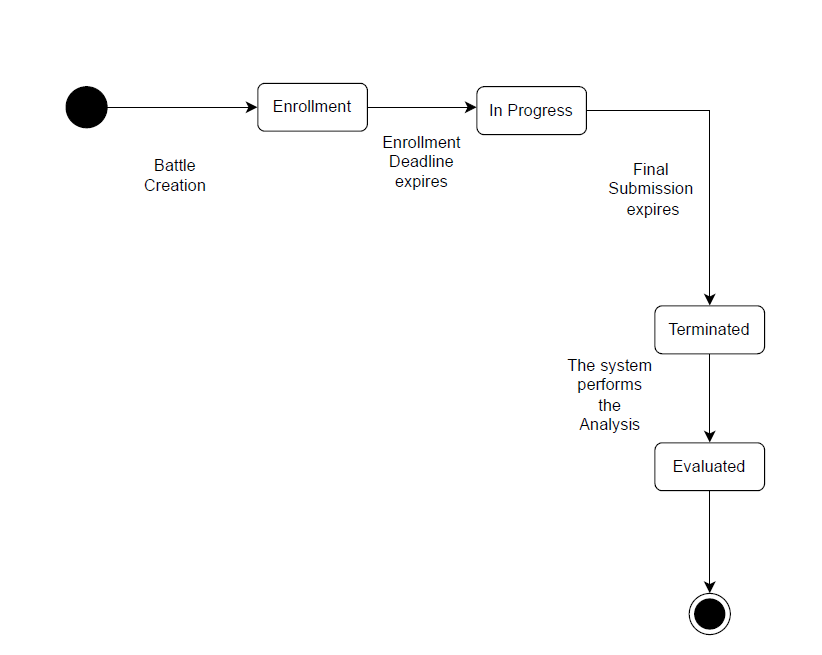
\includegraphics[width=12cm]{Images/startBattle.png}
\caption{Battle state charts}
\label{dcd}
\end{figure}

In this state chart diagram is explained how a battle works and the different states that it has. In the\textit{ Enrolment} state the students enrol in the battle and it is the very first state after the educator has created the battle.
The \textit{In progress} state represents the state in which the deadline for the enrollment has expired and the tournaments begins so the battle is going to be attended.The second-last state is \textit{Terminated} in which the battle is ended.The last state is  \textit{Evaluated} in which the system analysis has been performed and an evaluation has given either by the system or the educator.

\section{Product functions}
\subsubsection{Sign up and log in}
Sign-up is available to all users who want to subscribe to the platform. When a new user opens the platform, he will press the button 'Sign-in'. The user will then be redirected to GitHub \footnote{We decide to require users to use their GitHub account to sign. We already required students to have one to participate in the tournament, and this simplifies the process of checking who submitted the code, as each user is linked to one GitHub account. Also this decision could in the future allow us to seamlessly add more functionalities,  such as creating the web-hooks or forking the kata automatically and others that will ease the work of educators as well} where they are required to log in or create an account in order to link their GitHub account with our platform. Once this operation is completed, the platform will ask the user extra information, such as a username, so that the platform can create the user profile. Once the profile is created, the system allows the user to log into the platform for the first time using his GitHub account.\cite{githubOAuth}

\subsubsection{Tournament and battles management}
This function is only available to the educator. Their role is to create a tournament which consist of several battles that are related by the same topic. The first creator of the tournament allows his colleagues to contribute to the creation of the tournament by giving them the permission to add, modify, or delete battles for that tournament.
The teacher should provide the students with the necessary materials to do the kata and should also define the minimum and maximum number of students allowed for the battle. Finally, he should specify the deadlines for both registration to the battle and final submission of the code.

\subsubsection{Teams creation}
This function is available to all student who wants to create a team and join a battle. Once the team leader has signed up for the battle, it has the possibility to share an invitation link with other registered students. The students who received the invitation link can join the team-leader and subscribe to the battle.

\subsubsection{Scoring and ranking}
This function is available to any educator who wants to score and rank a group of students for their coding abilities. after a battle the educator has the possibility to manually evaluate the team that has uploaded the code based on some criteria.

\subsubsection{Badges}
This function allows educator to creates badges which are a reward for students achievements. The criteria to assign the badges are decided by the educator during the tournament creation.
Thanks to this function, every user can view the badges collected by each student by visiting their profile.

\subsubsection{Tournament and battles participation}
The students that are registered to the platform will receive a notification. Therefore, they can subscribe to the tournament after registering and will be informed of every incoming battle.
For what concerns each battle the students can form a team by using the platform they should create a repository on github if they do not create it, the platform will create it after the registration deadline.Then, the students have to fork the repository and they can start working on their project creating a workflow on github.Every push triggers the platform that starts doing the tests

\subsubsection{Tournament and battles consolidation}
This function allows the system to evaluate the code pushed by each team and assign it a score. This score is updated every time a new push is made into the repository.
When the battle ends, the educator who created the battle has the possibility to manually evaluate the code done by the teams for that battle by going through the sources implemented by the students. This phase is called consolidation because right after the manual evaluation the final score of the battle is calculated and all students who participate to it are notified about the ranking.

\section{User Characteristics}
There are mainly two types of user that interact with the platform: student and educator.

\subsection{Student}
The student  is able to register and login to the platform and is also allowed to participate to a tournament after the tournament if his performances will be good he will receive a badge based on the rules that he fulfilled

\subsection{Educator}
The educator is a user who can create a tournament and the battle inside of it.This type of user can also evaluate students after the battle and create a badge that will be assigned to students who had the best performances.



\pagebreak
\section{Assumptions, dependencies and constraints}

\subsection{Regulatory policies}
The CKB application asks for the GitHub account information. GitHub will not be used for commercial purposes. Personal information will be processed in compliance with the GPDR.

\subsection{Domain Assumptions}
The following assumptions are made for the domain. They are properties or conditions that the system will take for granted.They must be checked to ensure a correct platform behaviour
\begin{enumerate}[label={[D\arabic*]}]

    \item User must have a reliable internet connection
    \item User personal information must be correct
    \item Educators properly insert information about a tournament
    \item The Github interaction it's reliable( the user is able to pull and push the code without losing its data)
    \item Notifications to the user must arrive as soon as the final rank is available
    \item The Educator properly insert an evaluation manually when it's requested
    \item The educator correctly adds information about a new badge such as new rules or badge name
    
\end{enumerate}

%------------------------------------------------------------------------------------------------------------------------------------------------
\clearpage
{{\chapter{Specific Requirements}}}
\label{sect:requirements}
\section{External Interface Requirements}
\subsection{User Interfaces}
In this section is presented the UI of the web platform here are presented two type of user interfaces the one for the educator and the one for the student. The first one has the possibility to create tournaments and battles.
The second one has the possibility to compete inside a tournament and to receive some badges that shows the abilities that the student himself has consolidated by using the platform.Both the two types of users  need to insert their credentials to have access to the platform.Moreover a mechanism of forgot password it's needed just in case they lose their credentials. 
\subsection{Hardware Interfaces}
Our platform is a web app, as a consequence, it does not require any specific hardware interface except for computer and any other device with web browser.
\subsection{Software Interfaces}
In order to work the system needs some software  interfaces. Here they are listed in detail:
    \begin{itemize}
        \item Github API:In order to interact with github, for user login and registration as well as to create and manage repositories;
        \item Calendar API:it's useful to suggest to the user what battle it's going to happen;
        %\item Email notification:This API is useful because the user will receive a notification via email when a battle starts;
        \item Static analysis tool API: To evaluate the submitted code, we will send a request to the static tool with the code and then we expect an answer with the assigned score.
    \end{itemize}
\subsection{Communication Interfaces}
The user uses the internet connection to have access to the platform,to communicate with other user inside the platform and for pushing and pulling the code on github.The platform must be HTTPS compliant in order to work on the web properly and to be safe. 

\section{Functional Requirements}
%Definition of use case diagrams, use cases and associated sequence/activity diagrams, and mapping on requirements


\textbf{Sign up and log in}
\begin{enumerate}[label={[R\arabic*]}]
    
    \item The System allows users\footnote{users is used to refer to students and educators} to register by providing their personal information (Full Name, etc.), a valid email address and a password.
    \item The System allows registered user to log in
    \\  \\  \textbf{Tournament and battles management}
    \item The System allows Educators to create/modify a battle upload the code kata (description and software project, including test cases and build automation scripts)
    \item The System allows to create/modify/terminate a tournament by selecting the existing battles, setting the minimum and maximum number of students per group, the registration and final submission deadline.
    \item The System allows an educator to give or deny permission to his colleagues to modify a tournament.
    \item The System must notify subscribed user about upcoming battles and deadlines.
    \\  \\  \textbf{Student's teams}
    \item The System allows students to create a team
    \item The System allows students to invite other students into one of their teams
    \item The System allows students to join a new team which they were invited
    \\  \\  \textbf{Scoring and ranking}
    \item The system allows educators to define the scoring criteria for a specific battle which they have permissions to
    \item The system maintains and computes the scores of each battle
    \\ \\  \textbf{Badges}
    \item Educators can create a badge and a set of rules associated with that badge
    \item The system assigns the badges that are created by educators as a reward for the rules they fulfill
    \item The system shows the badges that are assigned to students

    \\  \\  \textbf{Tournament and battles participation}
    \item The System creates a repository on GitHub containing the code kata right after the registration deadline
    \item The system sends the link to all the enrolled students after creating the repository with the code kata
    \item The System receives notifications from GitHub regarding the students registered repositories commits
    \item The System pulls the repository after receiving a notification for that repository before the deadline of that battle
    \item The System runs the appropriate test on the new code after every pull of the repository
    \item The System calculate and update the team's score for that battle after rerunning the tests
    \\  \\  \textbf{Tournament and battles consolidation}
    \item The system updates the personal tournament score for each student enrolled in the tournament right after the battle ends
    \item The system allows educators to manually evaluate the code after the deadline
    \item The system  allows educators to finish the consolidation stage after completely performing the manual evaluation
    \item The system computes the final ranking of the tournament immediately after consolidation finishes
    \item The system  sends a notification about the tournament's termination to students 
\end{enumerate}

\subsection{Use cases Diagram}

\begin{wrapfigure}
    \centering
    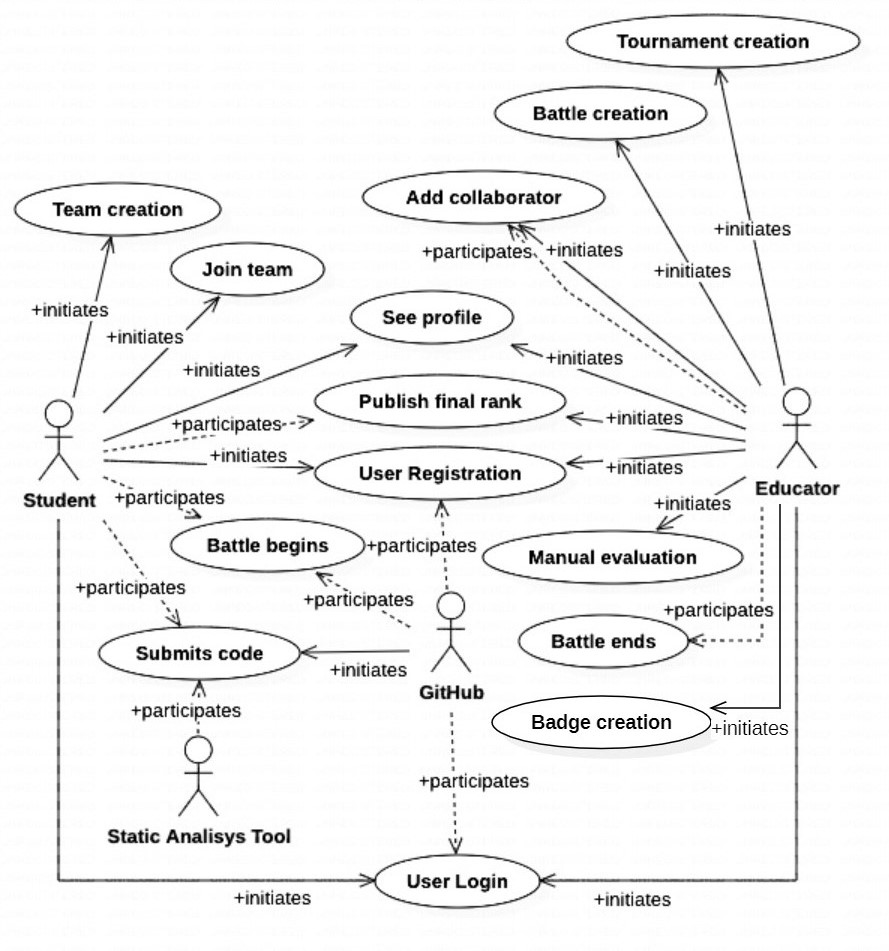
\includegraphics[width=15cm]{Images/ucd.jpg}
    \caption{Use cases diagram}
    \label{fig:enter-label}
\end{wrapfigure}

\subsection{Use cases}

\begin{enumerate}[label=\textbf{[UC\arabic*]}]
    \item \textbf{-User Registration}
    \\ \begin{tabular}{|l|p{11cm}|}
        \hline
        Name & User Registration \\
        \hline
        Actors & \begin{itemize}
                    \item user
                    \item GitHub
                \end{itemize} \\
        \hline
        Entry Condition & The user has opened the CKB platform\\
        \hline
        Event flow & \begin{enumerate} 
            \item The user press the button Sign-in
            \item The system redirect the user on GitHub to link their account to the platform
            \item The system shows a form to compile
            \item The user compile the form by adding a username
            \item The user press the button 'Register' to complete the registration
            \item The platform shows the login view
        \end{enumerate}\\
        \hline
        Exit condition & The user has successfully registered to the platform \\
        \hline
        Exception & \begin{enumerate} [label={}, leftmargin=0.25cm ]
            \item (d) There already exist a user with those credentials.
        \end{enumerate}  \\
        \hline            
    \end{tabular}
\newpage
    
 \item \textbf{-User Login}  
    \\ \begin{tabular}{|l|p{11cm}|}
        \hline
        Name & User Login\\
        \hline
        Actors & \begin{itemize}
                    \item user
                    \item GitHub
                \end{itemize} \\
        \hline
        Entry Condition & The user has opened the CKB platform\\
        \hline
        Event flow & \begin{enumerate}
            \item The user press the button Log-in
            \item The System redirect the user to GitHub platform to let him login to it, and checks the credentials
            \item The user is redirected to the platform with an access token
            \item The system shows the profile information
            \item The user presses the button 'Login'
            \item The platform shows the dashboard
        \end{enumerate}\\

        \hline
        Exit condition & The user has successfully accessed the service \\

        \hline
        Exception & \begin{enumerate} [label={}, leftmargin=0.25cm ]
            \item (c) The token is not valid. The platform will return to the entry condition
        \end{enumerate} \\ 
        \hline                
    \end{tabular}
    \pagebreak
   

\item  \textbf{-Tournament creation}
\\\begin{tabular}{|l|p{11cm}|}
        \hline
        Name & Tournament creation \\
        \hline
        Actors & \begin{itemize}
                    \item educator
                \end{itemize} \\
        \hline
        Entry Condition & The Educator is logged to the CKB platform\\
        \hline
        Event flow & \begin{enumerate}
            \item The educator goes to the tournament section
            \item The educator press the button to create a new tournament
            \item The system shows the educator the form to compile
            \item The educator fills the form with the information about the tournament:
            name, main context, enrolment deadline
            \item The educator press the button to submit the form
        \end{enumerate}\\
        \hline
        Exit condition & The educator has successfully created the tournament and returns to the tournament section  \\
        \hline
        Exception & \begin{enumerate} [label={}, leftmargin=0.25cm ]
            \item (d) The educator did not fill all the field of the form or they are not valid. The system will warn the user.
        \end{enumerate} \\
        \hline            
    \end{tabular}

\newpage
 \item \textbf{-Battle creation}
    \\ \begin{tabular}{|l|p{11cm}|}
        \hline
        Name & Battle Creation \\
        \hline
        Actors & \begin{itemize}
                    \item educator
                \end{itemize} \\
        \hline
        Entry Condition & The Educator is logged to the CKB platform and he already created a tournament\\
        \hline
        Event flow & \begin{enumerate}
            \item The educator goes to the tournament where he want to add the battle
            \item The educator press the button to create a new battle
            \item The system shows the educator the form to compile
            \item The educator fills the form with the information about the battle with the following information: battle name, code template, registration deadline, final submission deadline, sets minimum and maximum number of students per group that can participate in that battle and the scoring criteria for that battle
            \item The educator press the button to submit the form
        \end{enumerate}\\
        \hline
        Exit condition & The educator has successfully created the new battle and returns to the tournament main page \\
        \hline
        Exception & \begin{enumerate} [label={}, leftmargin=0.25cm ]
            \item (d) The educator did not fill all the field of the form or they are not valid. The system will warn the user. 
        \end{enumerate}\\
        \hline            
    \end{tabular}

\item \textbf{-Add collaborator}
    \\ \begin{tabular}{|l|p{11cm}|}
        \hline
        Name & Add collaborator\\
        \hline
        Actors & \begin{itemize}
                    \item educator
                \end{itemize} \\
        \hline
        Entry Condition & The educator is logged to the CKB platform and he is in the tournament section\\
        \hline
        Event flow & \begin{enumerate}
            \item The educator select the tournament
            \item The educator press the button to share the control of a tournament
            \item The system shows the educator a bar where to search other educators
            \item The educator can choose the other educators
            
        \end{enumerate}\\
        \hline
        Exit condition & The educator has successfully shared the access to the tournament control  \\
        \hline
        Exception & \begin{enumerate} [label={}, leftmargin=0.25cm ]
            \item (d) The educator did not make the correct choice
        \end{enumerate} \\
        \hline            
    \end{tabular}

\newpage
\item  \textbf{-Team creation}
    \\ \begin{tabular}{|l|p{11cm}|}
        \hline
        Name & Team creation \\
        \hline
        Actors & \begin{itemize}
                    \item student
                \end{itemize} \\
        \hline
        Entry Condition & The student is logged to the CKB platform and is enrolled into a tournament\\
        \hline
        Event flow & \begin{enumerate}
            \item The student goes to tournament section and selects the tournament
            \item The student select the battle for which create the team
            \item The student press the button create a team
            \item The system shows the student the form to compile
            \item The student fills the form with the information about the team: team name
            \item The system generate the link of the team 
            \item The student shares the link of the team with his friends
        \end{enumerate}\\
        \hline
        Exit condition &  The link team is successfully generated \\
        \hline
        Exception & \begin{enumerate} [label={}, leftmargin=0.25cm ]
            \item (c) The student has already created a team for that battle
        \end{enumerate} \\
        \hline            
    \end{tabular}

\item  \textbf{-Join team}
    \\ \begin{tabular}{|l|p{11cm}|}
        \hline
        Name & Join team  \\
        \hline
        Actors & \begin{itemize}
                    \item student
                \end{itemize} \\
        \hline
        Entry Condition & The student has the link to join a team\\
        \hline
        Event flow & \begin{enumerate}
            \item The student opens the link received
            \item The system checks the student's credentials
            \item The student press the button 'join the team'
            \item The system checks if the team is not full and that the student is not already enrolled in the battle
            \item The system redirect the student into the team dashboard
        \end{enumerate}\\
        \hline
        Exit condition &   The student has correctly joined the team \\
        \hline
        Exception & \begin{enumerate} [label={}, leftmargin=0.25cm ]
            \item (b) The student is not logged in, he will be redirect to the log in page
            \item (d) The system returns an error message
        \end{enumerate}\\ 
        \hline            
    \end{tabular}
\newpage
    \item  \textbf{-Battle begins}
    \\ \begin{tabular}{|l|p{11cm}|}
        \hline
        Name & Battle begins \\
        \hline
        Actors & \begin{itemize} 
                    \item student
                    \item GitHub
                \end{itemize} \\
        \hline
        Entry Condition & The enrollment deadline of the battle ended\\
        \hline
        Event flow & \begin{enumerate}
            \item The system creates a GitHub repository by using the appropriate API call for every enrolled team enrolled
            \item The system sends a notification to the students enrolled to the battle with the link to the specifically created repository for them to fork
        \end{enumerate}\\
        \hline
        Exit condition &   The code is available to all the students participating\\
        \hline
        Exception & \begin{enumerate} [label={}, leftmargin=0.25cm ]
            \item (b) The notification is not correctly sent, the system will retry to send it later.
        \end{enumerate}\\ 
        \hline            
    \end{tabular}

 \item  \textbf{-Submits code}
    \\ \begin{tabular}{|l|p{11cm}|}
        \hline
        Name & Student pushes the code \\
        \hline
        Actors & \begin{itemize}
                    \item student
                    \item GitHub
                    \item Static analysis tool
                \end{itemize} \\
        \hline
        Entry Condition & The student has forked to the git hub repository provided by the platform and set up the automated workflow. The student has committed the code into their GitHub repository\\
        \hline
        Event flow & \begin{enumerate}
            \item The system is triggered by GitHub about a new commit
            \item The system dynamically evaluates the code by running the test on it.
            \item The system send the code to the static analysis tool 
            \item The system receives the evaluation by the tool
            \item The system updates the score of the team.
        \end{enumerate}\\
        \hline
        Exit condition &   The scoring rank is correctly updated\\
        \hline
        Exception & \begin{enumerate} [label={}, leftmargin=0.25cm ]
             \item (a) The repository is not a fork of a code kata team, the system will ignore it and log it.
            \item (a) The system is triggered after the deadline of the battle, it will not evaluate the code and send a notification to the team warning them 
           
        \end{enumerate}\\ 
        \hline            
    \end{tabular}
\newpage
    \item  \textbf{-The battle ends}
    \\ \begin{tabular}{|l|p{11cm}|}
        \hline
        Name & The battle ends \\
        \hline
        Actors & \begin{itemize}
                    \item educator
                \end{itemize} \\
        \hline
        Entry Condition & the battle deadline has expired \\
        \hline
        Event flow & \begin{enumerate}
            \item The system creates the rank of the battle
            \item The system sends a notification the the educators enrolled into the battle about the end of it
        \end{enumerate}\\
        \hline
        Exit condition & The ranking is available on the platform \\
        \hline
        Exception & \begin{enumerate} [label={}, leftmargin=0.25cm ]
            \item (b) The notification is not correctly sent, the system will notify it and retry to send it
        \end{enumerate}\\ 
        \hline            
    \end{tabular}

        \item  \textbf{-Code evaluation}
    \\ \begin{tabular}{|l|p{11cm}|}
        \hline
        Name & The code is evaluated \\
        \hline
        Actors & \begin{itemize}
                    \item educator
                \end{itemize} \\
        \hline
        Entry Condition & The tournament ended, the consolidation phase started and the educator is logged to the CKB platform\\
        \hline
        Event flow & \begin{enumerate}
            \item The educator goes to the tournament section
            \item The educator select the tournament which needs a manual evaluation
            \item The educator reads the sources produced by the teams
            \item The educator assign a score to each student enrolled to the battle
        \end{enumerate}\\
        \hline
        Exit condition &  The system stores the score provided by the educator\\
        
        \hline            
    \end{tabular}
\newpage
        \item  \textbf{-Publish final rank}
    \\ \begin{tabular}{|l|p{11cm}|}
        \hline
        Name & Final rank made available \\
        \hline
        Actors & \begin{itemize}
                    \item student
                    \item educator
                \end{itemize} \\
        \hline
        Entry Condition & The tournament is in consolidation phase, the educator is logged to the CKB platform \\
        \hline
        Event flow & \begin{enumerate}
            \item The educator goes to the tournament section
            \item The educator selects the tournament to close
            \item The educator press the button 'close the tournament'
            \item The system computes the final rank for each student enrolled into the tournament
            \item The system notifies the student about the availability of the rank
            \item The system checks among the participating students who satisfied the badges requirement
            \item The system assign the badge to the students
        \end{enumerate}\\
        \hline
        Exit condition &  The final rank is published, and badges has been assigned \\
        \hline
        Exception & \begin{enumerate}  [label={}, leftmargin=0.25cm ]
            \item (c) If any student does not have a manual evaluation and it was required then an error message will be shown.
            \item (e) The notification is not correctly sent, the system will notify it and retry to send it
        \end{enumerate}\\ 
        \hline            
    \end{tabular}


        \item  \textbf{-See profile}
    \\ \begin{tabular}{|l|p{11cm}|}
        \hline
        Name & see profile \\
        \hline
        Actors & \begin{itemize}
                    \item user
                \end{itemize} \\
        \hline
        Entry Condition &  The user is logged to the CKB platform\\
        \hline
        Event flow & \begin{enumerate}
            \item The user search the name of the student
            \item The system shows the list
            \item The user selects the Student
        \end{enumerate}\\
        \hline
        Exit condition & The platform shows the rank of the selected student  
        \\
        \hline
        Exception & \begin{enumerate} [label={}, leftmargin=0.25cm ]
            \item (a) The person searched  does not match with any user in the system. It shows a no student found message
        \end{enumerate}\\ 
        \hline            
    \end{tabular}

\newpage


 \item \textbf{-Badge creation}
    \\ \begin{tabular}{|l|p{11cm}|}
        \hline
        Name & Badge Creation \\
        \hline
        Actors & \begin{itemize}
                    \item educator
                \end{itemize} \\
        \hline
        Entry Condition & The educator is logged to the CKB platform and he already created a tournament\\
        \hline
        Event flow & \begin{enumerate}
            \item The educator goes to tournament section
            \item The educator goes to the tournament where he want to add the badge
            \item The educator press the button to create a new badge
            \item The system shows the educator the form to compile
            \item The educator fills the form with the information about the badge with the following information: badge name and the rule which has to comply with the syntax specified $^2$
            \item The educator press the button to submit the form
        \end{enumerate}\\
        \hline
        Exit condition & The educator has successfully created the new badge and returns to the tournament main page \\
        \hline
        Exception & \begin{enumerate} [label={}, leftmargin=0.25cm ]
            \item (e) The educator did not fill all the field of the form or they are not valid  (e.g. the rule is invalid). The system will warn the user. 
        \end{enumerate}\\
        \hline            
    \end{tabular}
\footnote{More details on the rules syntax will be provided in the DD}

\newpage

\subsection{Sequence diagrams}

\begin{enumerate}[label=\textbf{[UC\arabic*]}]

    \begin{figure}[!h]
    \item \textbf{User Registration}
    \centering
    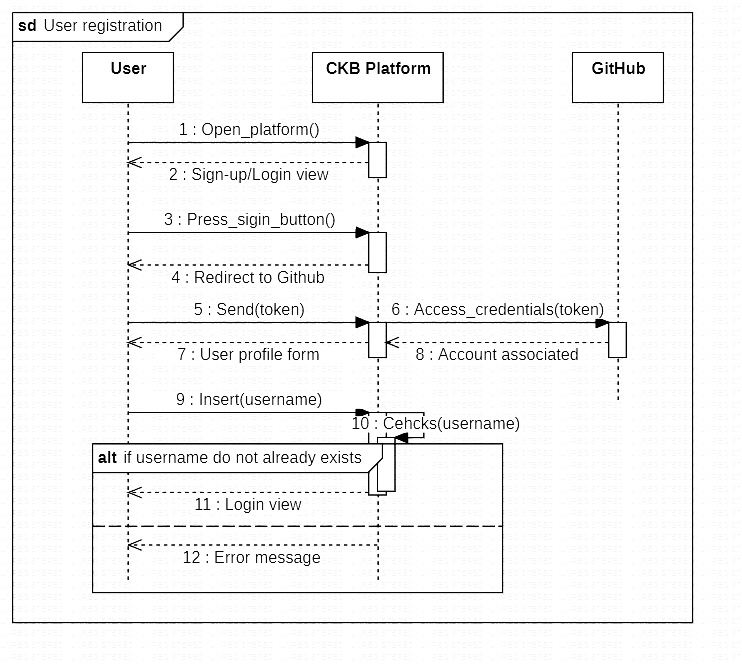
\includegraphics[width=\textwidth]{Images/User registration.jpg}
    \caption{User Registration}
    \label{fig:enter-label}
    \end{figure}

    \begin{figure}
    \item \textbf{User Login}
    \centering
    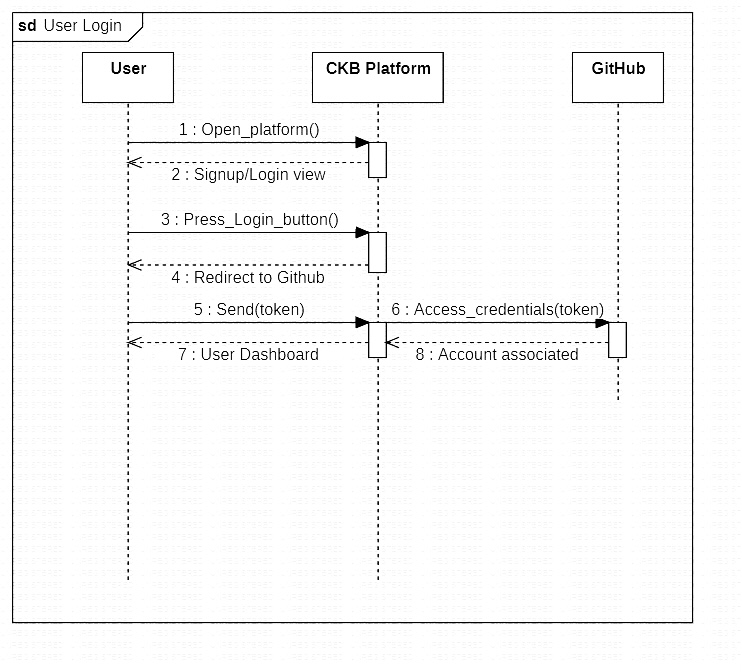
\includegraphics[width= \textwidth]{Images/User login.jpeg}
    \caption{User Login}
    \label{fig:enter-label}
    \end{figure}



    \begin{figure}
    \item \textbf{Tournament Creation}
        \centering
        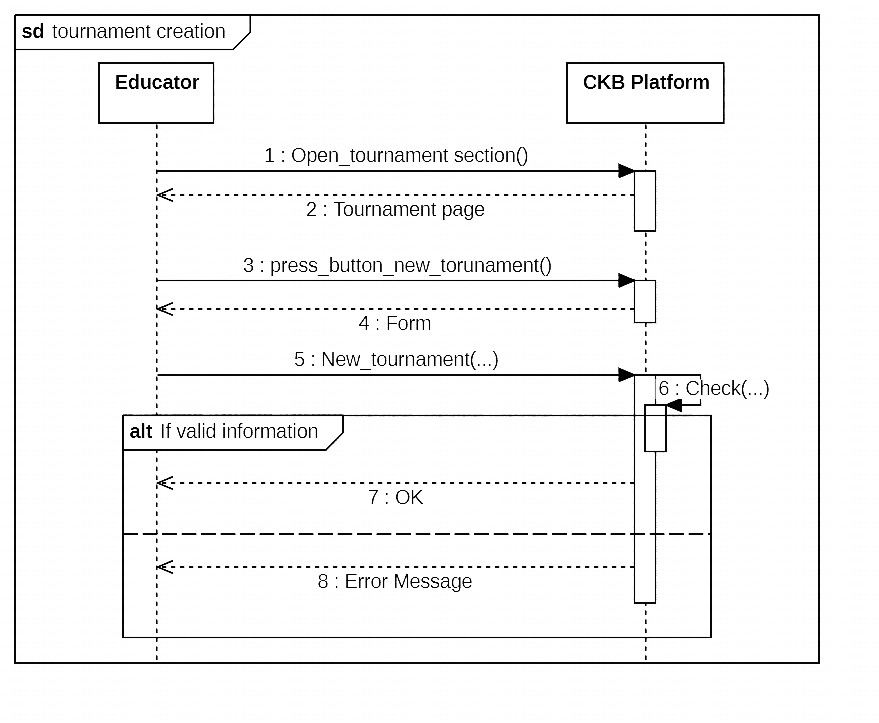
\includegraphics[width= \textwidth]{Images/Tournament creation.jpg}
        \caption{Tournament Creation}
        \label{fig:enter-label}
    \end{figure}
    
    
    \begin{figure}
    \item \textbf{Battle Creation}
        \centering
        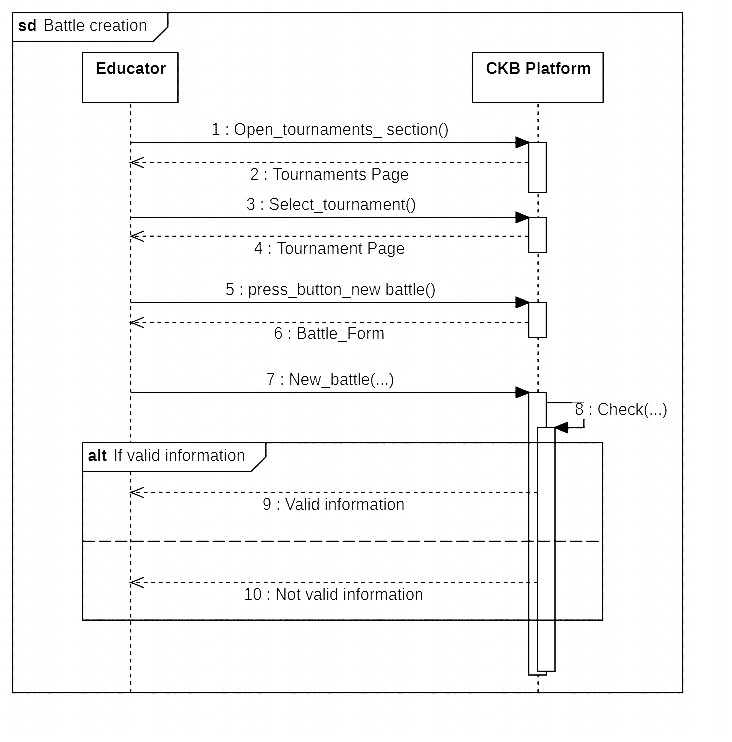
\includegraphics[width= \textwidth]{Images/Battle creation.jpg}
        \caption{Battle Creation}
        \label{fig:enter-label}
    \end{figure}
    
    \begin{figure}
    \item \textbf{Add collaborator}
        \centering
        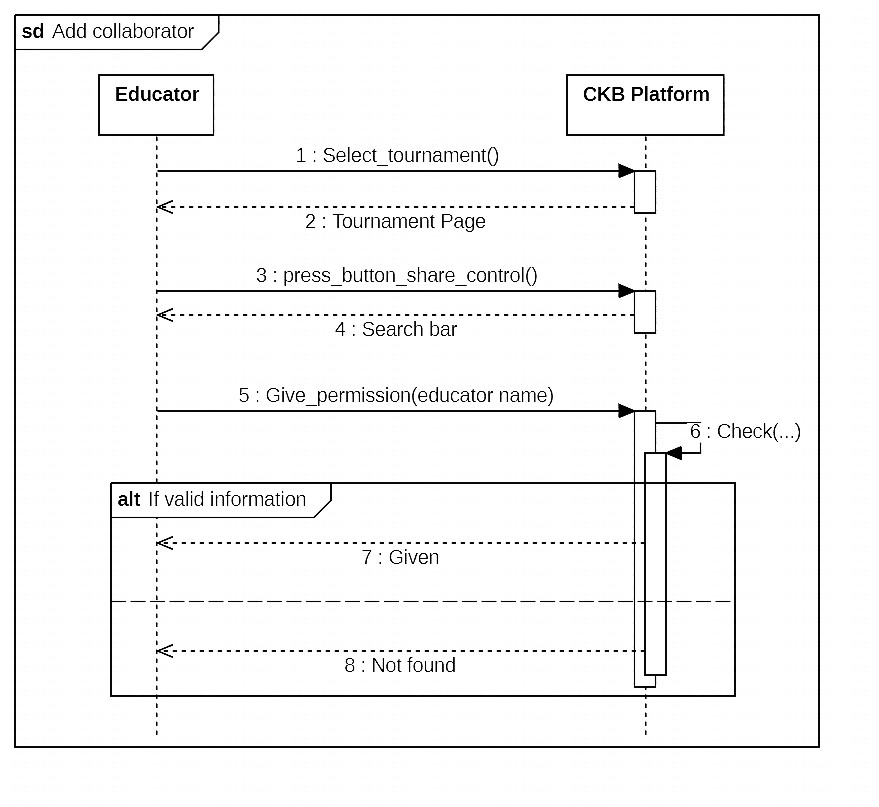
\includegraphics[width= \textwidth]{Images/Add collaborator.jpg}
        \caption{Add collaborator}
        \label{fig:enter-label}
    \end{figure}
    
    
    \begin{figure}
    \item \textbf{Team Creation}
        \centering
        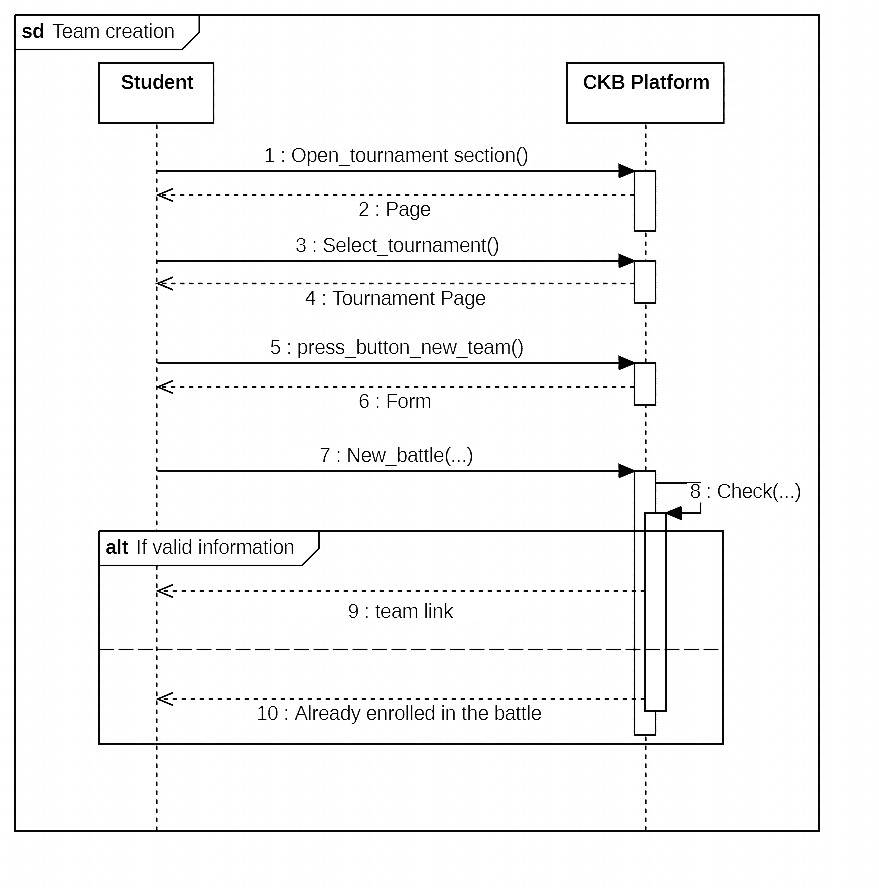
\includegraphics[width= \textwidth]{Images/Team creation.jpg}
        \caption{Team Creation}
        \label{fig:enter-label}
    \end{figure}
    
    \begin{figure}
    \item \textbf{Join Team}
        \centering
        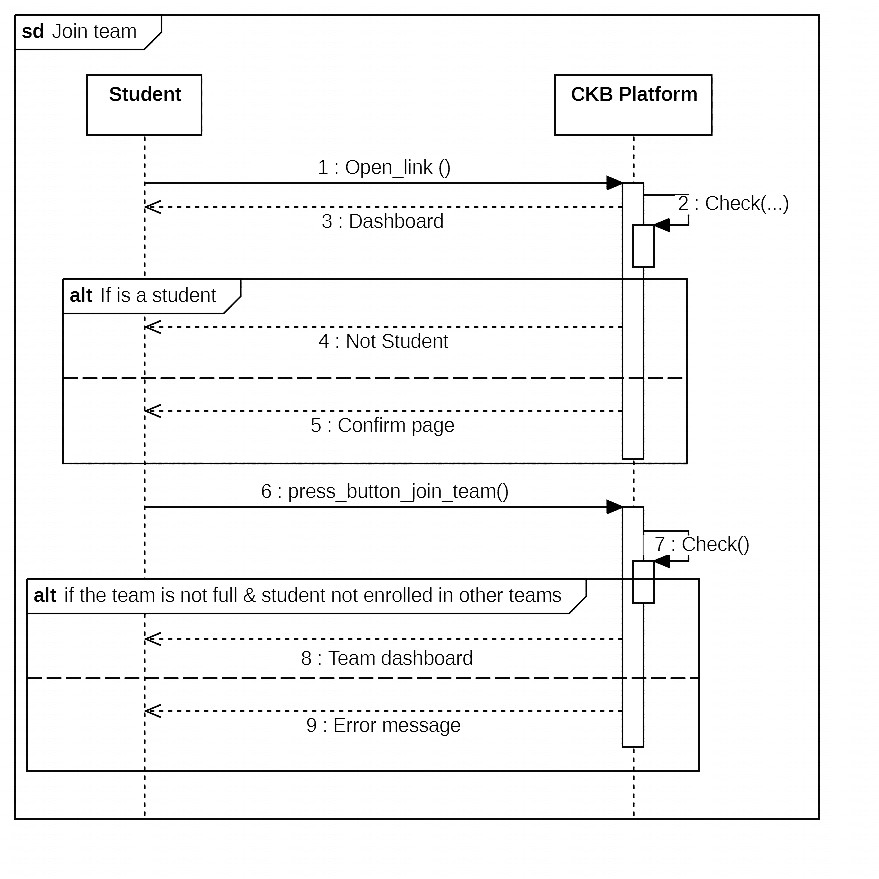
\includegraphics[width= \textwidth]{Images/Join team.jpg}
        \caption{Join Team}
        \label{fig:enter-label}
    \end{figure}
    
    \begin{figure}
    \item \textbf{Battle Begins}
        \centering
        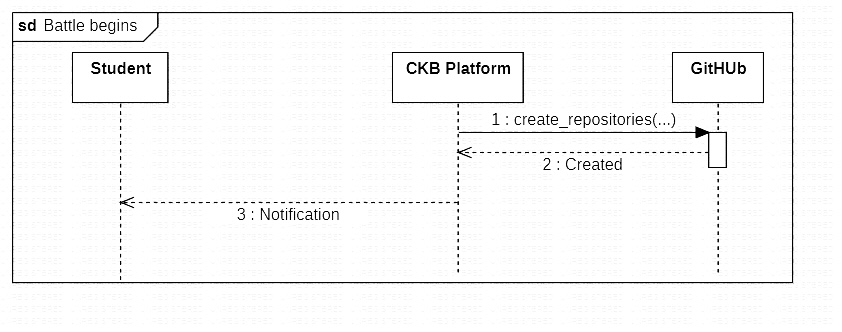
\includegraphics[width= \textwidth]{Images/Battle begins.jpg}
        \caption{Battle Begins}
        \label{fig:enter-label}
    \end{figure}
    
    \begin{figure}
    \item \textbf{Submits code}
        \centering
        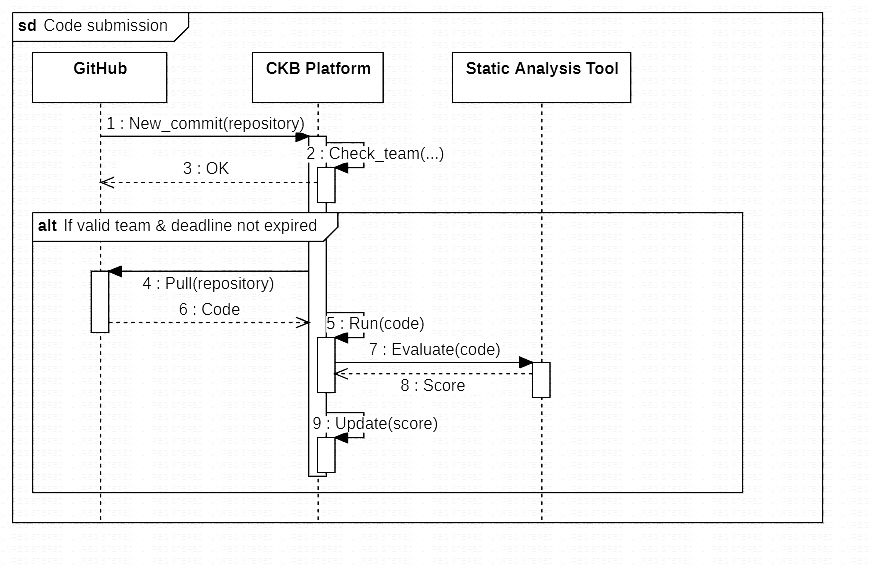
\includegraphics[width= \textwidth]{Images/Code submission.jpg}
        \caption{Submits Code}
        \label{fig:enter-label}
    \end{figure}

    \begin{figure}
    \item \textbf{The battle ends}
        \centering
        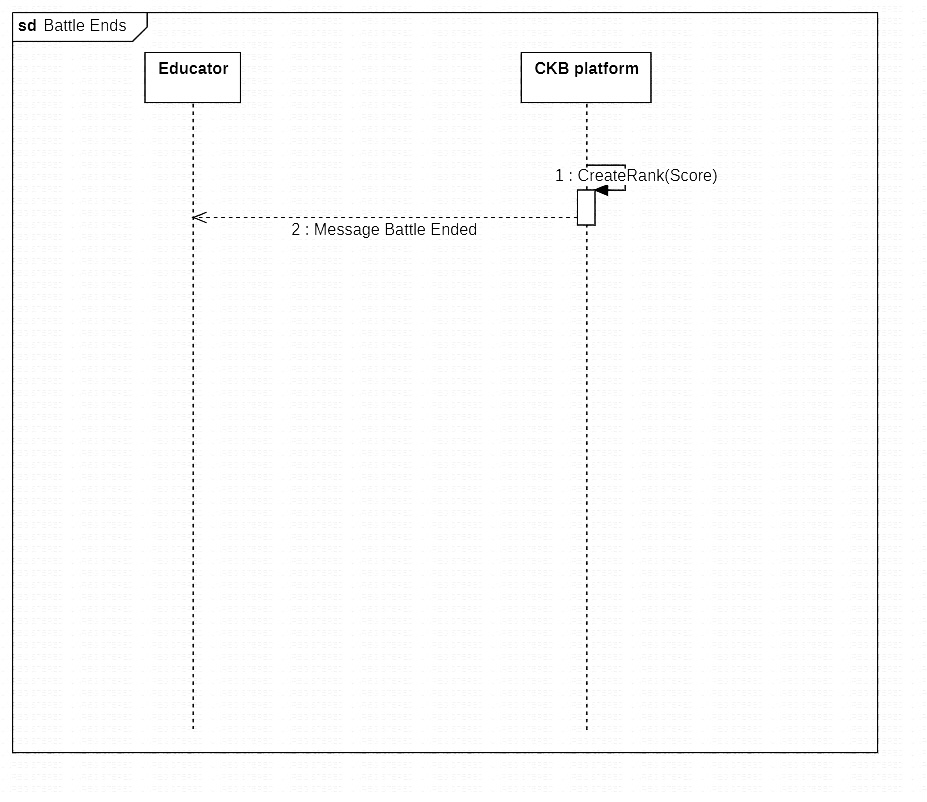
\includegraphics[width= \textwidth]{Images/Battle Ends.jpg}
        \caption{The battle ends}
        \label{fig:enter-label}
    \end{figure}
    
    \begin{figure}
    \item \textbf{Code Evaluation}
        \centering
        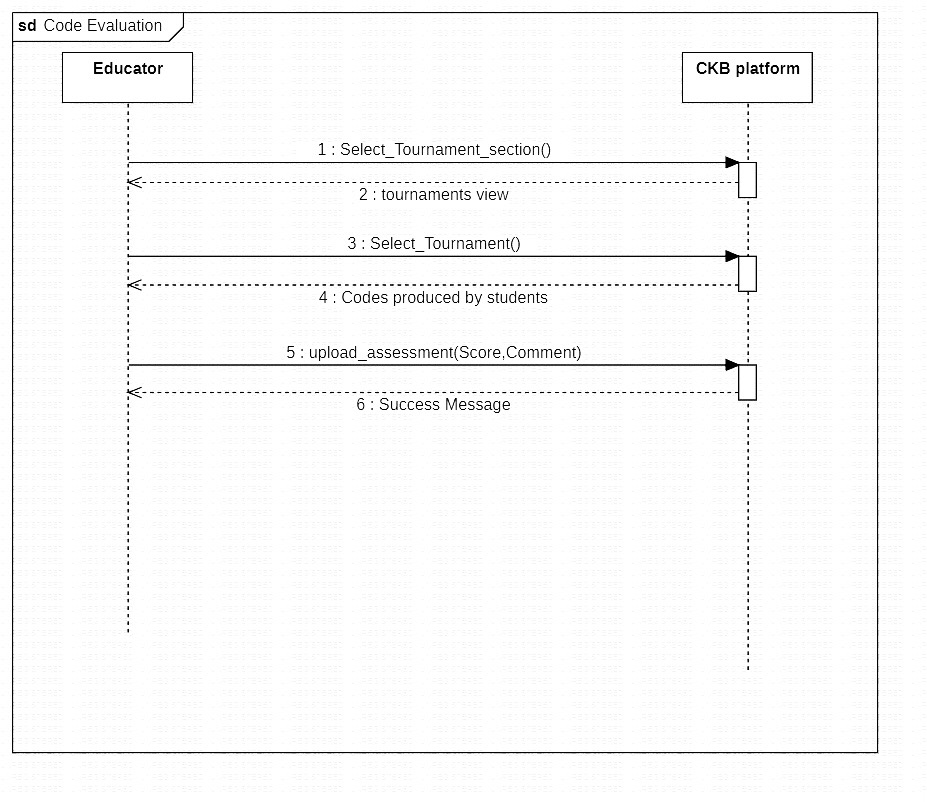
\includegraphics[width= \textwidth]{Images/f4c0a22a-3bab-4ba7-8605-08f8577774b5}
        \caption{Code Evaluation}
        \label{fig:enter-label}
    \end{figure}
    
    \begin{figure}
    \item \textbf{Publish Final Rank}
        \centering
        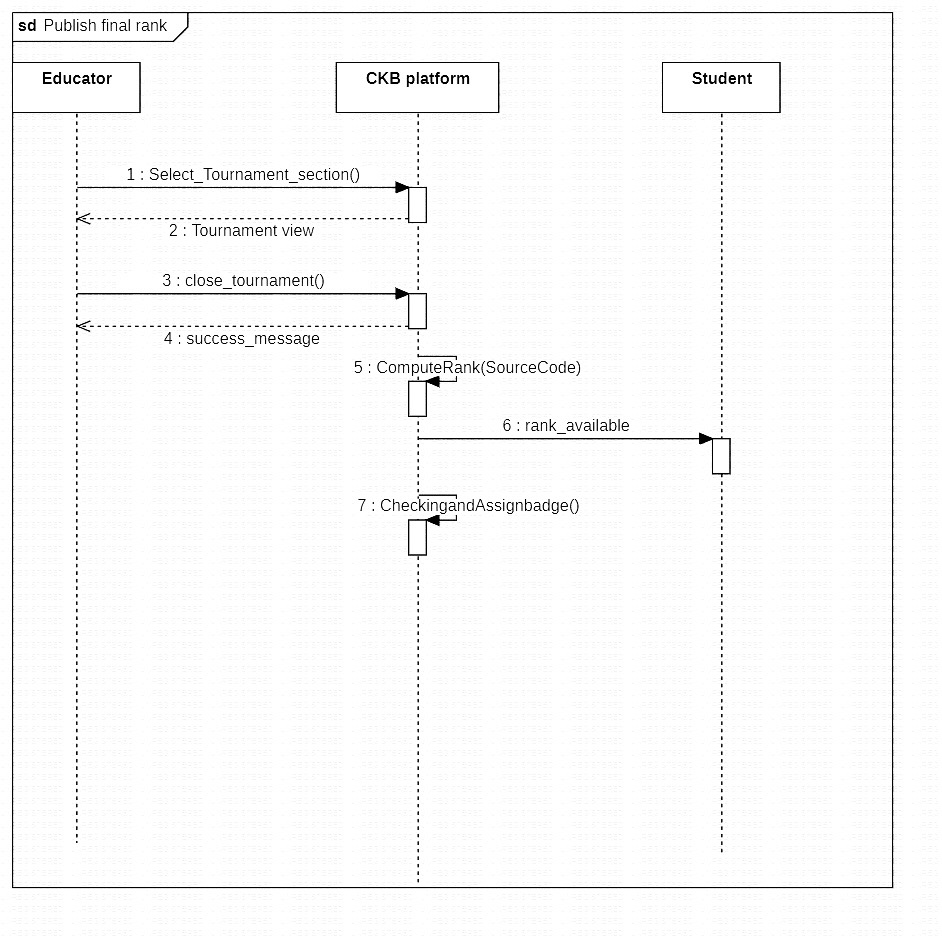
\includegraphics[width= \textwidth]{Images/e08ea53b-0385-4fb7-8284-6672fda72856}
        \caption{Publish Final Rank}
        \label{fig:enter-label}
    \end{figure}

    \begin{figure}
    \item \textbf{See Profile}
        \centering
        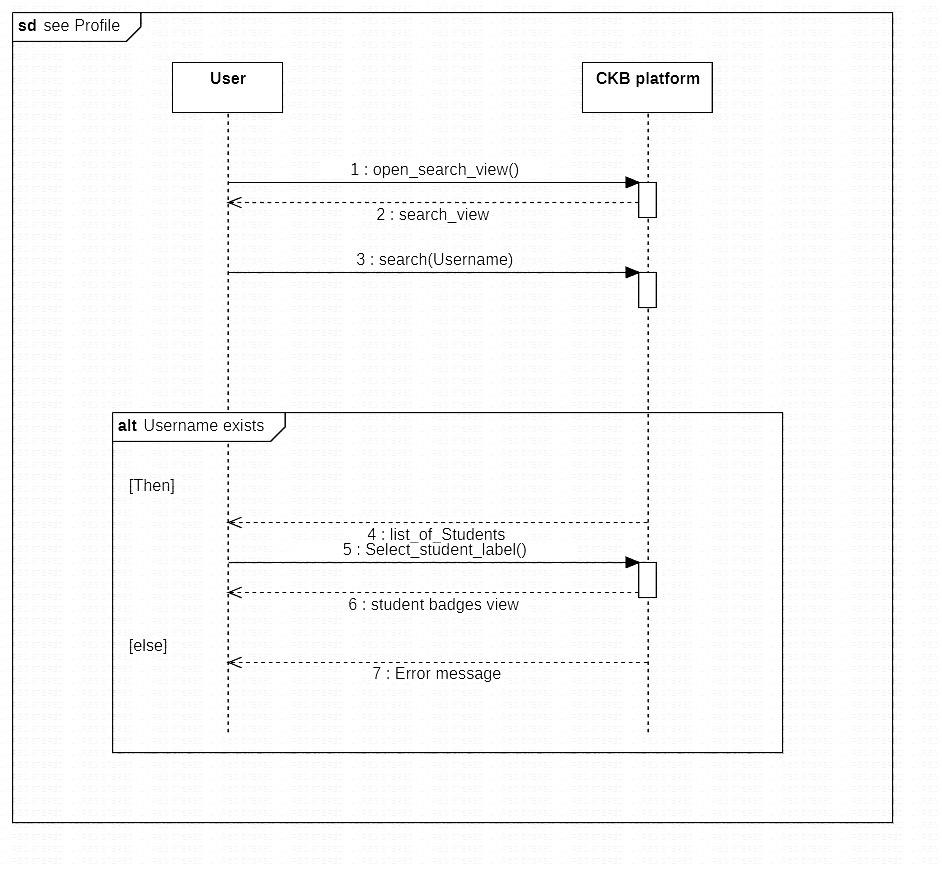
\includegraphics[width= \textwidth]{Images/WhatsApp Image 2023-12-20 at 18.34.43_e728ecf8.jpg}
        \caption{See Profile}
        \label{fig:enter-label}
    \end{figure}

    \begin{figure}
    \item \textbf{Badge Creation}
        \centering
        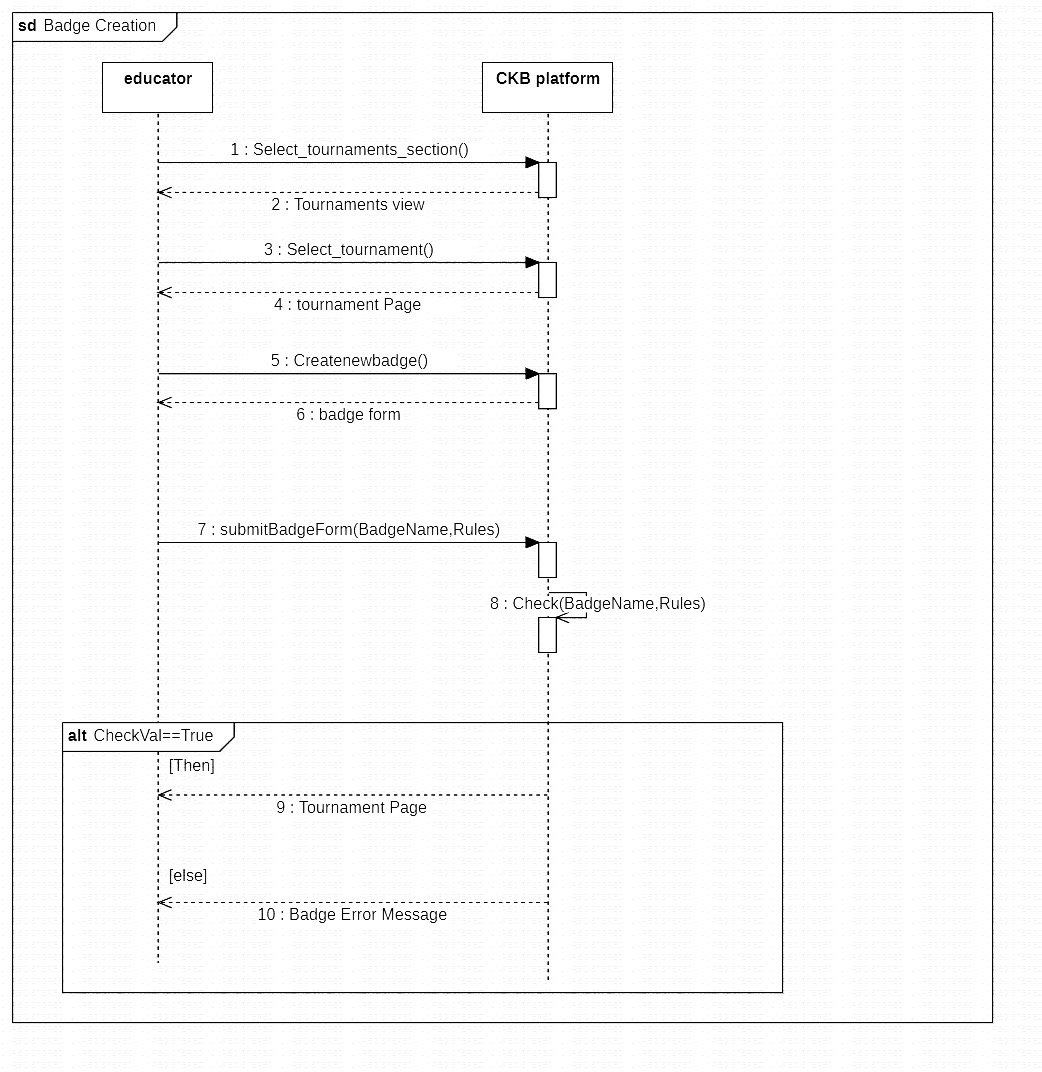
\includegraphics[width= \textwidth]{2058f325-4760-4dfa-ad83-44ce21cc7063}
        \caption{Badge Creation}
        \label{fig:enter-label}
    \end{figure}

    

    
    
\end{enumerate}








\pagebreak[4]
\newpage

\subsection{Requirement mapping}
\begin{tabular}{|p{7cm}|p{7cm}|}
\hline
\multicolumn{2}{|c|}{
\textbf{[G1] Educators create code kata battles} }
\\
\hline
\begin{itemize} 
\item [R1] The System allows users1 to register by providing their personal information (Full Name, etc.), a valid email address and a password
\item [R2] The System allows registered user to log in
\item [R3] The System allows Educators to create/modify a battle upload the code kata (description and software project, including test cases and build automation scripts)
\item [R4] The System allows to create/modify/terminate a tournament by selecting the existing battles, setting the minimum and maximum number of students per group, the registration and final submission deadline.
\item [R5] The System allows an educator to give or deny permission to his colleagues to modify a tournament.
\item [R10] The system allows educators to define the scoring criteria for a specific battle which they have permissions to
\item [R11] The system maintains and computes the scores of each battle
\item [R12] Educators can create a badge and a set of rules associated with that badge
\end{itemize}
&
\begin{itemize}
    \item [D1] User must have a reliable internet connection
    \item [D2] User personal information must be correct
    \item [D3] Educators properly insert information about a tournament
    \item [D7] The educator correctly adds information about a new badge such as new rules or badge name
\end{itemize}
\\
\hline
\end{tabular}

\pagebreak

\begin{tabular}{|p{7cm}|p{7cm}|}
\hline
\multicolumn{2}{|c|}{
\textbf{[G2] Students compete in multiple tournaments in teams} }
\\
\hline
\begin{itemize}
    \item [R1] The System allows users to register using a github acccount
    \item [R2] The System allows registered user to log in
    \item [R6] The System must notify subscribed user about upcoming battles and deadlines.
    \item [R7] The System allows students to create a team
    \item [R8] The System allows students to invite other students into one of their teams
    \item [R9] The System allows students to join a new team which they were invited
    \item [R15] The System creates a repository on GitHub containing the code kata right after the registration deadline
    \item [R16] The system sends the link to all the enrolled students after creating the repository with the code kata
    \item [R17] The System receives notifications from GitHub regarding the students registered repositories commits
    \item [R18] The System pulls the repository after receiving a notification for that repository before the deadline of that battle
    \item [R19] The System runs the appropriate test on the new code after every pull of the repository
    \item [R20] The System calculate and update the team's score for that battle after rerunning the tests
    \item [R25] The system  sends a notification about the tournament's termination to students
\end{itemize}
&
\begin{itemize}
    \item [D1] User must have a reliable internet connection
    \item [D2] User personal information must be correct
    \item [D4] The Github interaction it's reliable( the user is able to pull and push the code without losing its data)
    \item [D5] Notifications to the user must arrive as soon as the final rank is available
\end{itemize}
\\
\hline
\end{tabular}

\begin{tabular}{|p{7cm}|p{7cm}|}
\hline
\multicolumn{2}{|c|}{
\textbf{[G3] Students receive performance feedback after each battle assessment}}
\\
\hline
\begin{itemize}
    \item [R10] The system allows educators to define the scoring criteria for a specific battle which they have permissions to
    \item [R11] The system maintains and computes the scores of each battle
    \item [R12] Educators can create a badge and a set of rules associated with that badge
    \item[R13] The system assigns the badges that are created by educators as a reward for the rules they fulfill
    \item [R14] The system shows the badges that are assigned to students 
    \item [R20] The System calculate and update the team's score for that battle after rerunning the tests
    \item [R21] The system updates the personal tournament score for each student enrolled in the tournament right after the battle ends
    \item [R22] The system allows educators to manually evaluate the code after the deadline
    \item [R23] The system  allows educators to finish the consolidation stage after completely performing the manual evaluation
    \item [R24] The system computes the final ranking of the tournament immediately after consolidation finishes
\end{itemize}
&
\begin{itemize}
    \item [D4] The Github interaction it's reliable( the user is able to pull and push the code without losing its data)
    \item [D5] Notifications to the user must arrive as soon as the final rank is available
    \item [D6] The Educator properly insert an evaluation manually when it’s requested
    \item [D7] The educator correctly adds information about a new badge such as new rules or badge name
\end{itemize}
\\
\hline
\end{tabular}



\section{Performance Requirements}
The system has to guarantee good performances in order to serve a great number of users (educators and students).To achieve this goal the user experience must be as good as possible in order to fulfill this requirement the response time must be low no more than a second.If the user’s internet connection is slow the response time can increase  enormously

\section{Design Constraints}

\subsection{Standards compliance}
The CKB platform pays a great attention for what concerns users privacy cause of this the CKB project is in compliance with the  General Data Protection Regulation
(GPDR) a regulation in EU law on data protection and privacy for all
individuals within the European Union (EU) and the European Economic Area (EEA).
Moreover, the platform has to use the international format of date and time to adequate to the newer standards.
\subsection{Hardware limitations}
Here is presented a summary of the hardware features that a user should have to use the platform properly:
    \begin{enumerate}[label=\textbullet]
        \item The user must have a device with a good internet connection for providing this the device should be compatible with at least one of this standards 3G, 4G, 5G, IEEE 802.11 and  IEEE 802.3. Both for the wired and wireless communications it must be connected to a device able to guarantee an internet connection such as a modem or an access point and so on;
        \item The user must have a device with good hardware features such as a processor with high performance as an example intel i5 or i7 and a display with high resolution at least full hd and a fair amount of ram at least 8 GB.
        
    \end{enumerate}



    


\subsection{Any other constraint}
The UI should be user-friendly because the CKB platform is developed for educators and students that are learning to code. Furthermore, they must be able to use the platform in a simple and efficient way.

\section{Software System Attributes}
Here are explained some  software side attributes that the system should provide.
\subsection{Reliability}
The system has to be reliable because it will have to run continuously for a long period of time.
To ensure this feature the platform must have some sort of replication and consistency policy to avoid system crash. Moreover, as best practice, it is important to have offline backups of the system for recovering information after data loss.
\subsection{Availability}
The most important attribute that the system has to provide is the availability. The system should have an availability of 99\%.Since the platform has to achieve this goal some replication policies must be implemented and a single point of failure should be avoided. Also it has to be specially prepared for a possibly large amount of submissions when deadline is close.
\subsection{Security}
The system will store the users personal data so the security aspect must be carefully considered. Passwords stored in the central database must be encrypted.
The data store must be protected with all possible security measures to avoid internal and external attacks. The CKB platform must ensure integrity, consistency and confidentiality by using appropriate cyber-risk avoidance policies.
Additionally, because students code will be ran on the system for the dynamic analysis, a proper way to do these has to be explored making sure no malicious code can  damage the platform.
\subsection{Maintainability}The system must guarantee a good level of maintainability. The code has to be well documented. A testing routine has to be provided and it has to cover at least 75\% of the entire code excluding the UI code.
\subsection{Portability}
The system is a web application so it must be compatible with different web browser (Firefox,Google Chrome and so on) and devices (smartphones, computers, etc).





%------------------------------------------------------------------------------------------------------------------------------------------------
\clearpage
{{\chapter{Formal Analysis Using Alloy}}}
\label{sect:alloy}
For the alloy part we focused on modelling the ranking of a tournament ($T$) and see how it evolves after groups submit their code.
We also analyse different properties of the ranking ($R_{t,T}$) a relation that establishes which student ($s\in S$) ranks better or equal depending on their score and their current submissions($R_{t,T}\subseteq S\times S$).

\begin{lstlisting}[language=alloy]
open util/relation
open util/boolean


sig Tournament {}

//A battle has to belong to exactly one tournament
sig Battle {
	belongsTo: one Tournament
}

sig Student {}

//A group is a team of students for a specific battle
sig Group {
	participants: set Student,
	battle: Battle
} { participants !=none and cannotEnrollTwiceInABattle }

//We rename it for clarity
sig Score in Int {}
 
//The submission it is of a specific group and has associated a score
//To represent that submissions are submitted over time we added the submited attribute
sig Submission {
	group: one Group,
	score: one Score,
	var submited: one Bool
}{ score>=0 and score<=100 }
//Here we capture the fact that student can enroll only once to any battle if not it would be unfair
pred cannotEnrollTwiceInABattle {
	all disj g,h:Group | g.participants&h.participants=none or g.battle!=h.battle
}


//Auxiliary functions used to compute the score:

//Retrieves all the submissions of a group
fun submissions [g:Group]:set Submission{
	(group:>g).dom
}

//Retrieves only the submited ones of a group
fun effectiveSubmissions [g:Group]:set Submission{
	{s:g.submissions | s.submited.isTrue}
}

//Calculates all the obtained scores of a group until that moment
fun scores [g:Group]: set Score{
	g.effectiveSubmissions.score
}

//The best score of a group if it has not submitted it is 0
fun bestScore [g:Group]: Score {
	max[g.scores + {0}]
}

//The participants of a tournament in this case it is not necessary to have submitted jus to be enrolled (be part of a group in any of the battles belonging to it)
fun participants[t:Tournament]:Student {
	{s:Student | (some g:Group | t=g.battle.belongsTo and s in g.participants)}
}

//Score of the student only considering the scores obtained in the battles belonging to it
fun scoreInTournament[s:Student, t:Tournament]: Int{
	sum g:s.groupsForATournament[t] | g.bestScore
}

//For the prevoius we need to retrieve the groups in which the student participates related to the tournament
fun groupsForATournament[s:Student, t:Tournament]: set Group {
	{g:Group | s in g.participants and t=g.battle.belongsTo }
}

//Returns the ranking relation for a tournament as previously explained
fun ranking[t:Tournament]: Student -> Student {
	{b,w: t.participants | int b.scoreInTournament[t]>= int w.scoreInTournament[t]}
}


//To model correctly the evolution of the competition we add the following facts:

//The competition begins with 0 effective submissions
fact noSubmissionsAtStart {
		all s:Submission| s.submited.isFalse
}

//It ends after all the generated submissions become effective
pred allTournamentsEnd {
	eventually all s:Submission| s.submited.isTrue
}
fact {allTournamentsEnd}

//Each step can only submit one submission
pred submit [s:Submission]{
	submited' = submited ++ s->True
}
fact oneSubmissionPerStep {
	always some s:Submission| s.submit
}

\end{lstlisting}

\section{Examples}
\begin{figure}[h]
\caption{A simple example with two submissions to see if the behavior is the expected one}

\centering
\begin{lstlisting}[language=alloy]
run {} for 5 but exactly 2 Submission, 9 int
\end{lstlisting}

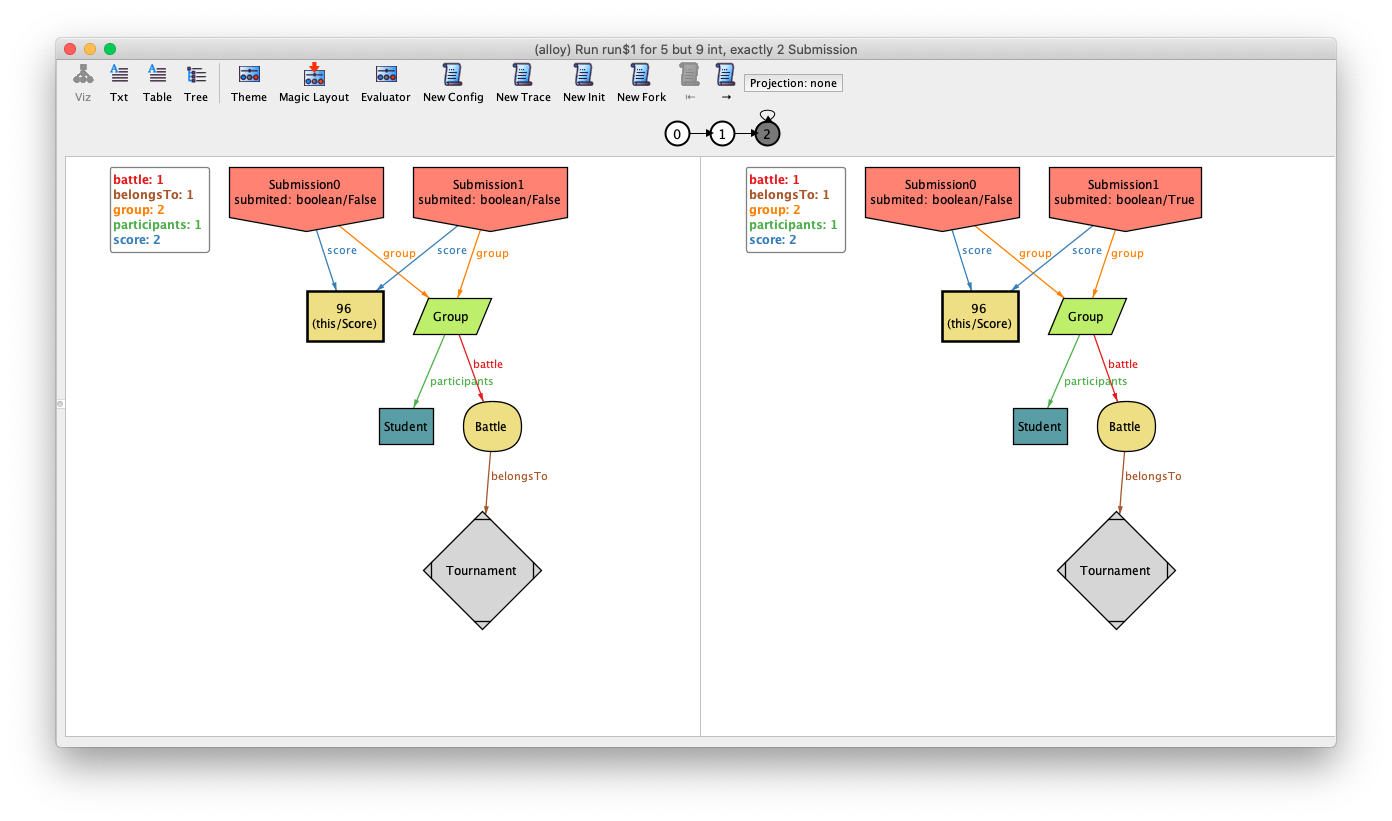
\includegraphics[width=\textwidth]{Images/First example 1.png}
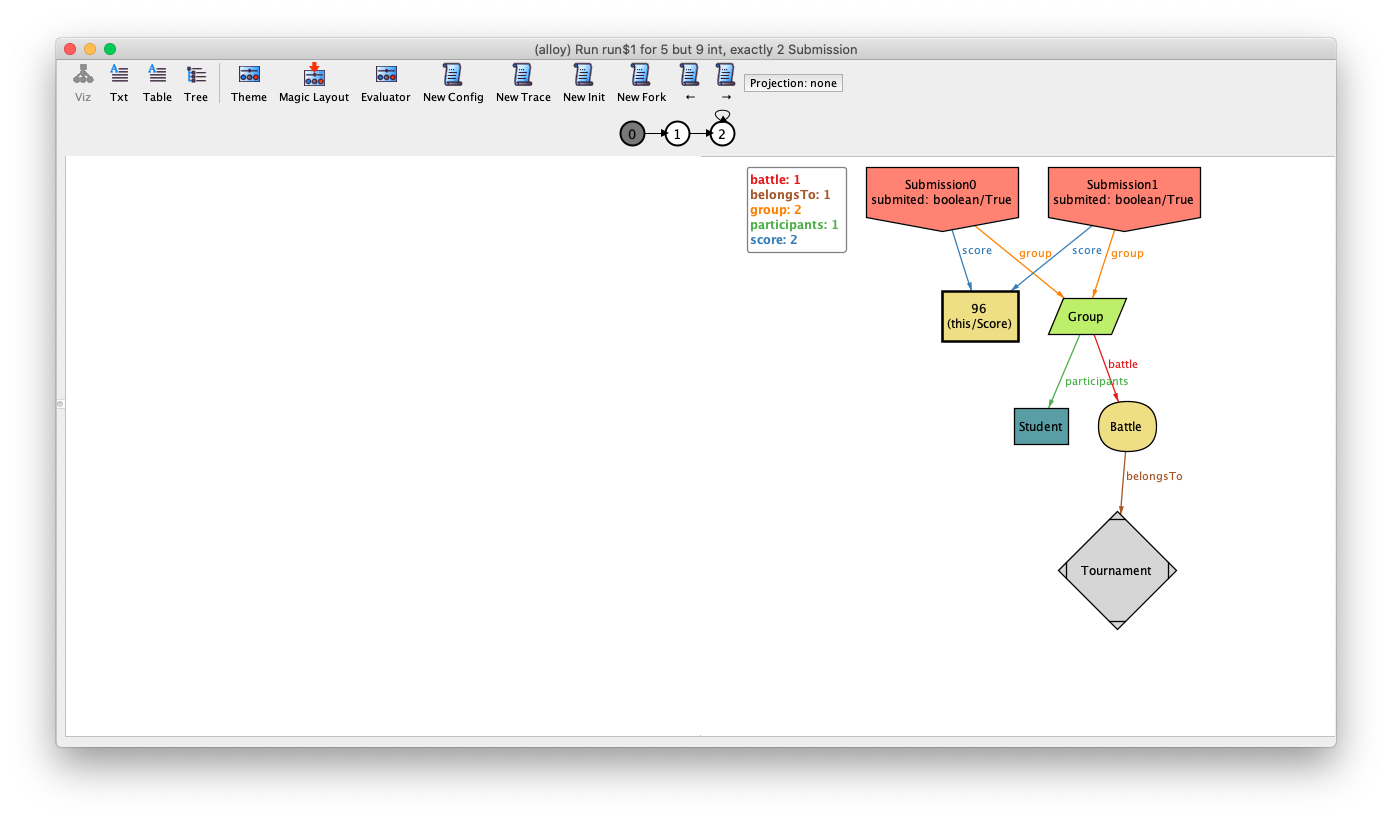
\includegraphics[width=\textwidth]{Images/First example 2.png}

\end{figure}

\begin{figure}[h]
\caption{An example where the final ranking is a relation of total order (i.e. with no ties and everyone participates)}

\centering
\begin{lstlisting}[language=alloy]
run {
	eventually some t:Tournament |  totalOrder[t.ranking,Student] 
} for 3 but exactly 1 Tournament, exactly 3 Student, 9 int
\end{lstlisting}

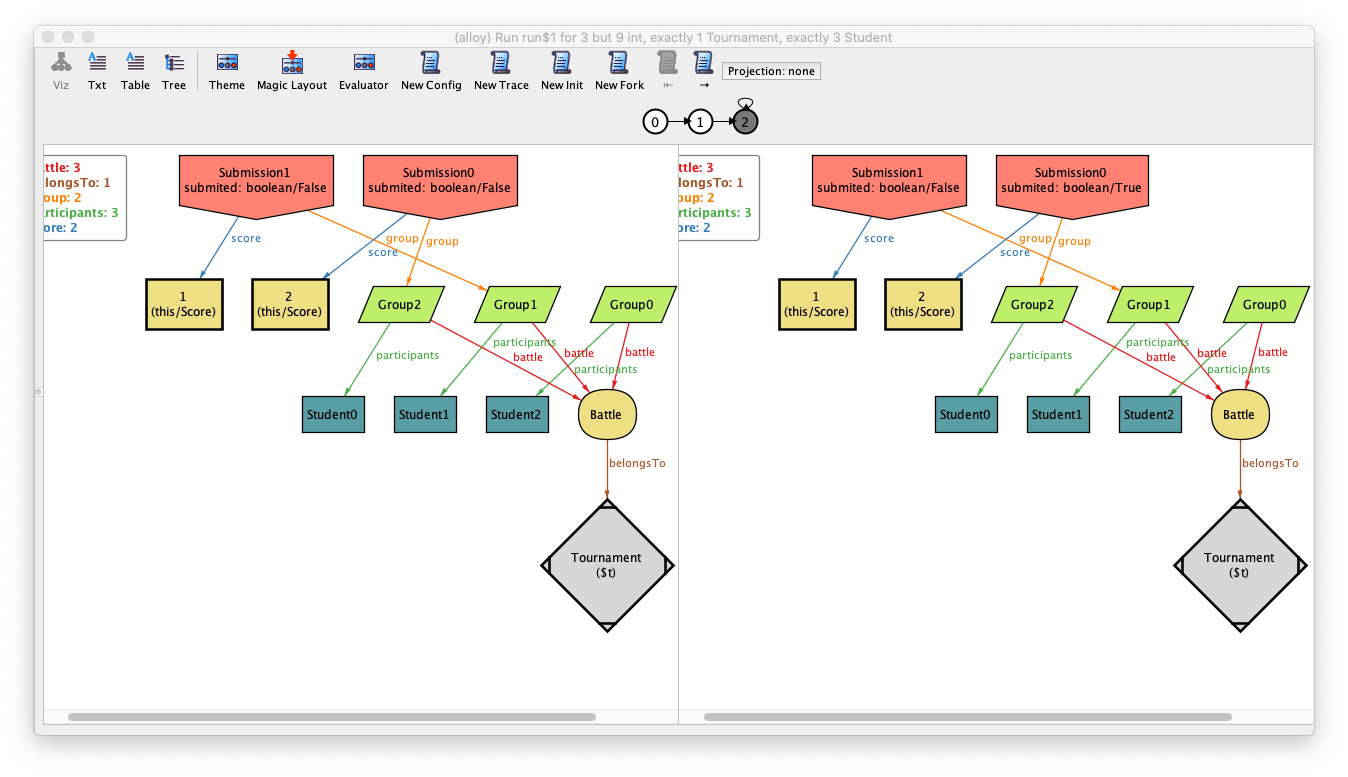
\includegraphics[width=\textwidth]{Images/Second example 1.png}
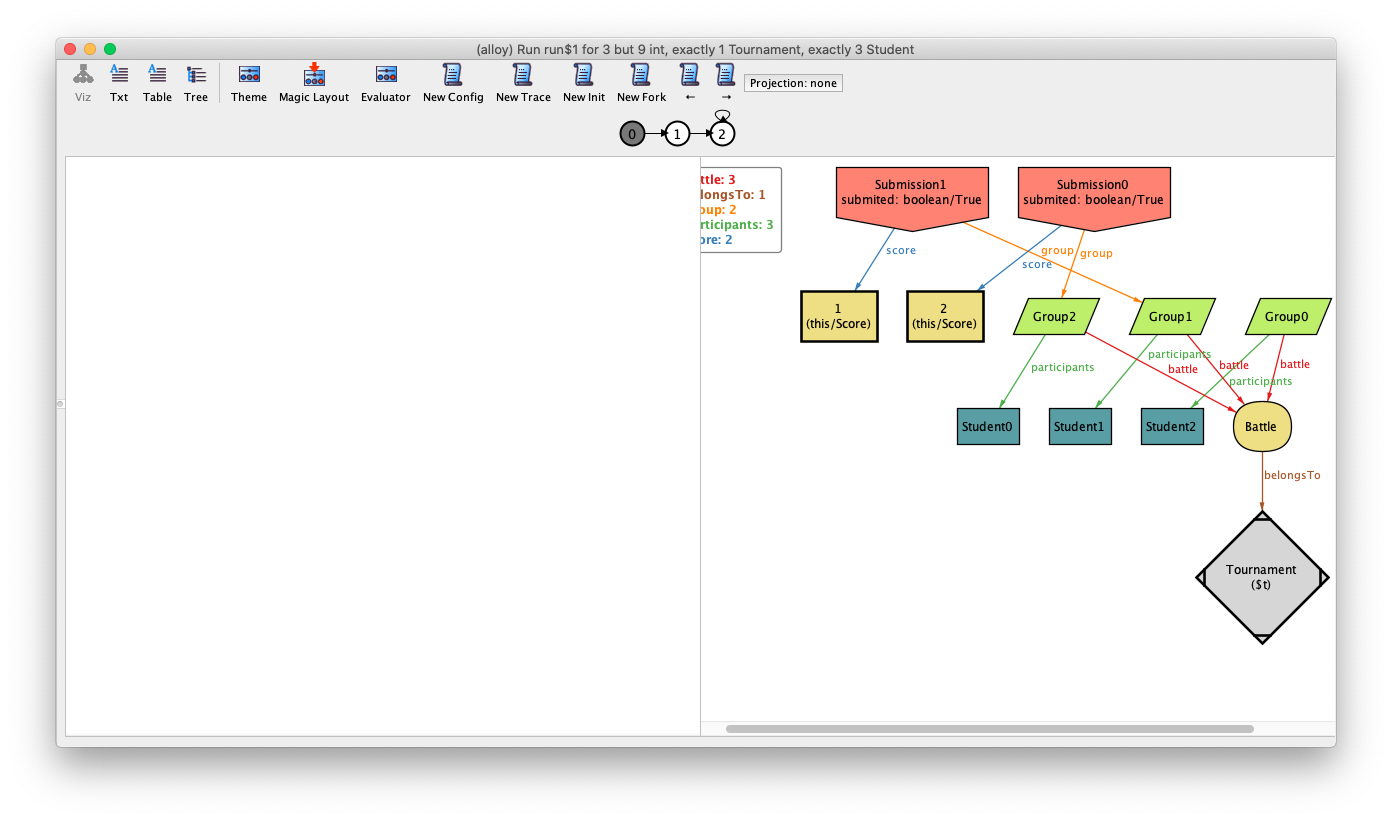
\includegraphics[width=\textwidth]{Images/Second example 2.png}
Final ranking:


\begin{tabular}{c|c}
    Student & Score \\
    \hline
    0 & 2 \\
    1 & 1 \\
    2 & 0 \\
\end{tabular}
\end{figure}


\begin{figure}[h]
\caption{Counterexample to prove that ranking is not always a partial order (neither a total order)  because of ties.}

\centering
\begin{lstlisting}[language=alloy]
check {
	after  all t:Tournament | partialOrder[t.ranking,t.participants]
}  for 9 Int
\end{lstlisting}

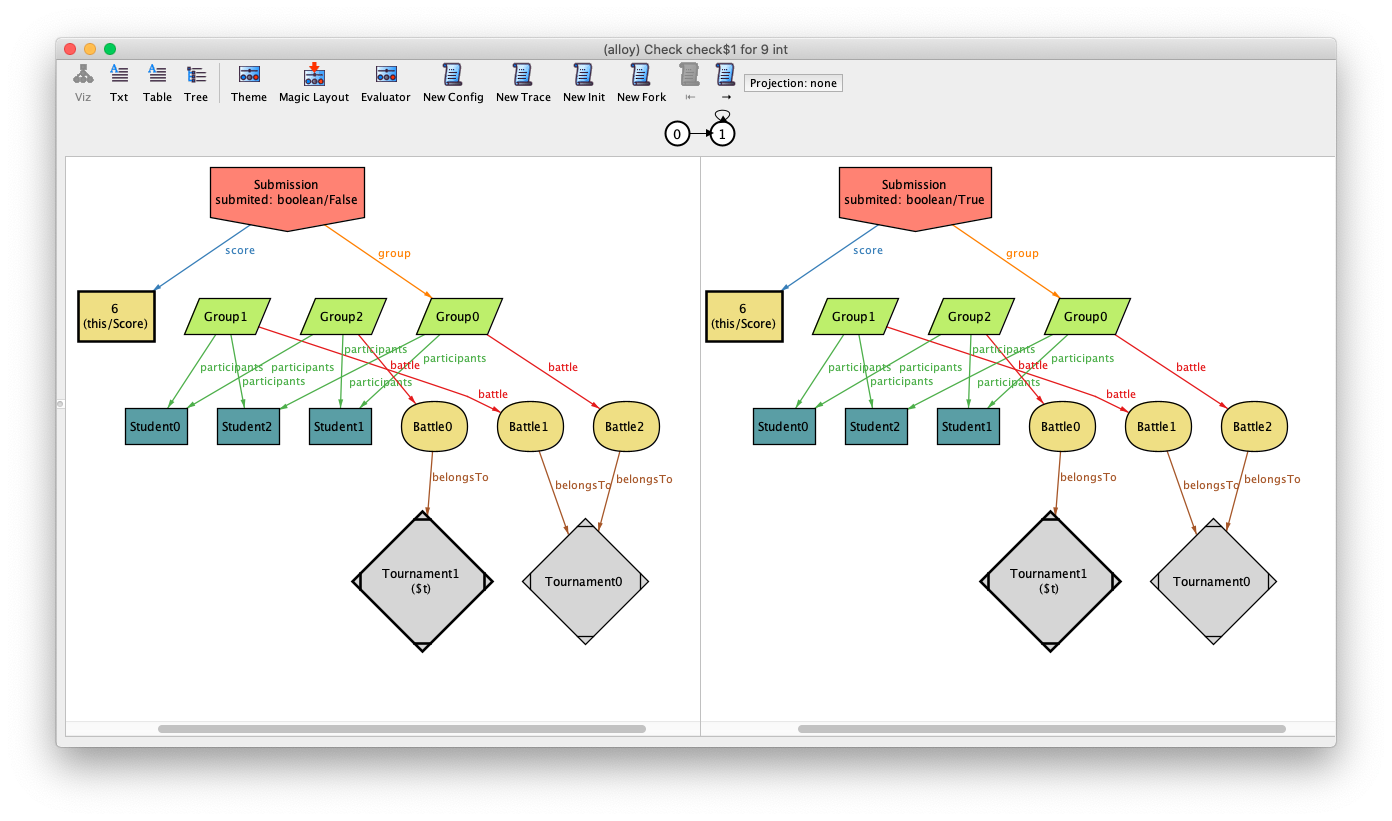
\includegraphics[width=\textwidth]{Images/Counterexample.png}
Final ranking for \$t:

\begin{tabular}{c|c}
    Student & Score \\
    \hline
    0 & 0 \\
    1 & 0 \\
\end{tabular}
\end{figure}

\begin{figure}[h]
\caption{Check that ranking is a preorder}

\centering
\begin{lstlisting}[language=alloy]
check {
	after all  t:Tournament |  preorder[t.ranking,t.participants]
} for 9 Int
\end{lstlisting}

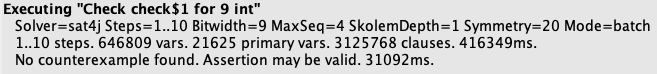
\includegraphics[width=\textwidth]{Images/Correct.png}
\end{figure}

\begin{figure}[h]
\caption{Simple example to show that a student can improve his score and tie the best one}

Because the relation has only 2 participants: the ranking relation is symmetric $\leftrightarrow$ there is a tie
\centering
\begin{lstlisting}[language=alloy]
run {
	eventually some  t:Tournament | #t.participants=2 and symmetric[t.ranking];
	some  t:Tournament | antisymmetric[t.ranking];
	some  t:Tournament | symmetric[t.ranking]
} for 3 but exactly 2 Student, 1 Tournament, 9 int
\end{lstlisting}

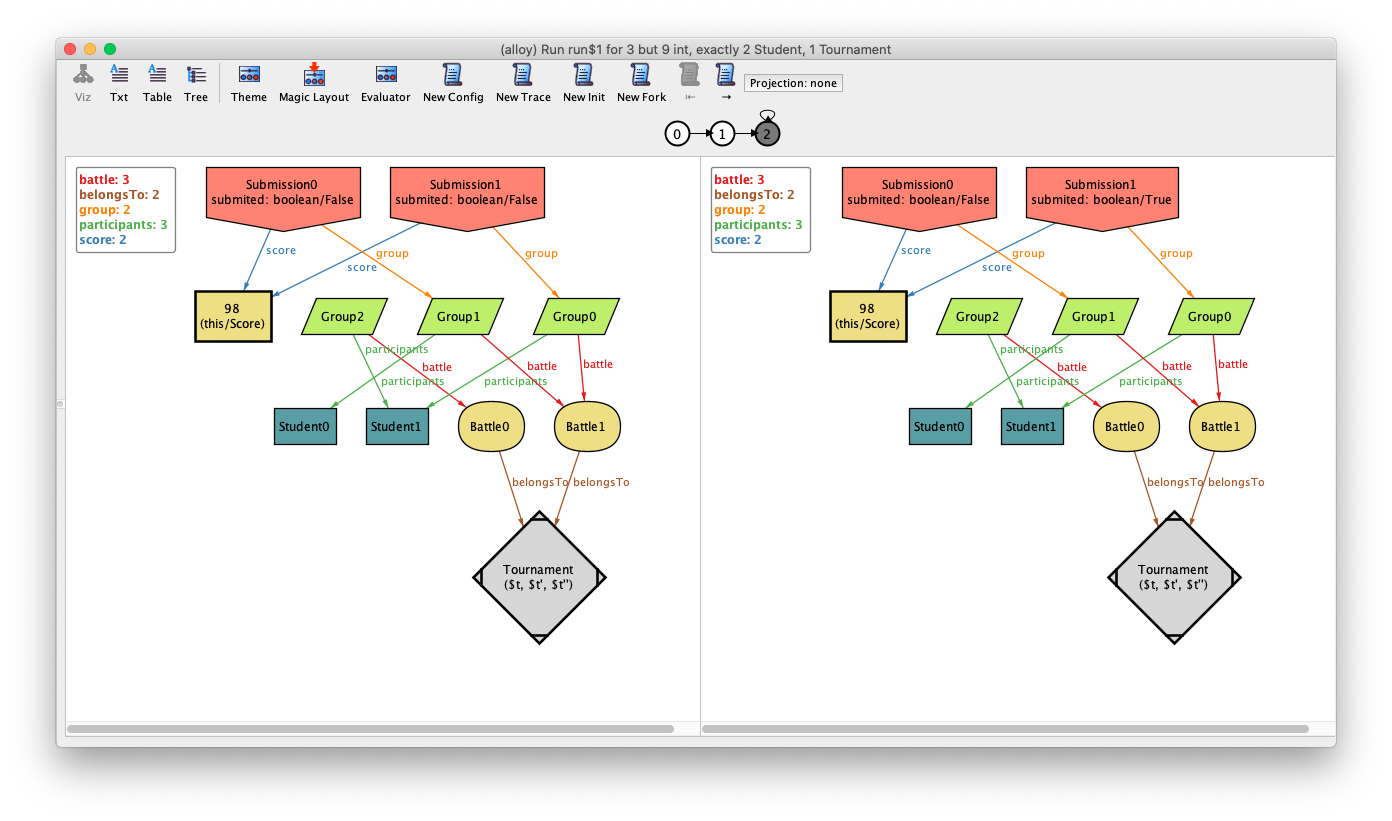
\includegraphics[width=\textwidth]{Images/Last example 1.png}
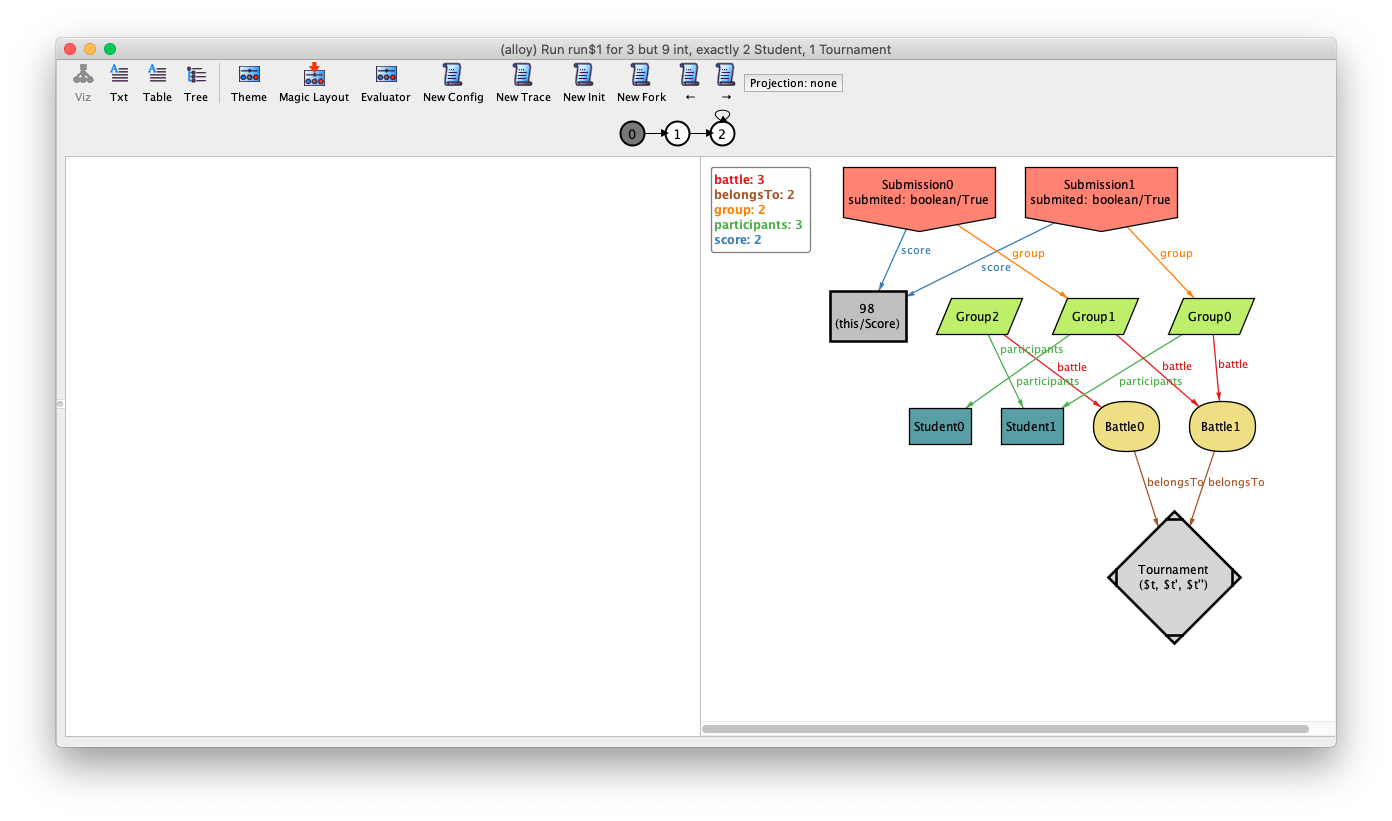
\includegraphics[width=\textwidth]{Images/Last example 2.png}
Ranking evolution:

\begin{tabular}{c||c|c|c}
    Student & Score & Score' & Score''\\
    \hline
    1 & 0 & 98 & 98\\
    0 & 0 & 0 & 98\\
\end{tabular}

\end{figure}

%------------------------------------------------------------------------------------------------------------------------------------------------
\clearpage
\chapter{Effort Spent}
\label{sect:effort}
In this part there is an overview of the time effort spent by each member of this team. Everyone have spent some time writing each section of this document and here its visible the amount of time.\\
\begin{itemize}
    

\item  \textbf{Andaloro Emanuele}
\begin{table}[h!]
    \centering
    \begin{tabular}{|c|p{10cm}|}
        \hline
        \textbf{chapter} & \textbf{Effort(In hours)} \\
        \hline
        1 & 5 \\
        \hline
        2 & 10\\
        \hline
        3 & 25\\
        \hline
        4 & 3\\
        \hline            
    \end{tabular}
    \end{table}

\item  \textbf{Deveali Lew Simon}
\begin{table}[h!]
    \centering
    \begin{tabular}{|c|p{10cm}|}
        \hline
        \textbf{chapter} & \textbf{Effort(In hours)} \\
        \hline
        1 & 5 \\
        \hline
        2 & 10\\
        \hline
        3 & 10\\
        \hline
        4 & 18\\
        \hline            
    \end{tabular}
    \end{table}

\item  \textbf{Galantino Claudia}
\begin{table}[h!]
    \centering
    \begin{tabular}{|c|p{10cm}|}
        \hline
        \textbf{chapter} & \textbf{Effort(In hours)} \\
        \hline
        1 & 5 \\
        \hline
        2 & 16\\
        \hline
        3 & 20\\
        \hline
        4 & 2\\
        \hline            
    \end{tabular}
    \end{table}    

\end{itemize}


%-------------------------------------------------------------------------
%	BIBLIOGRAPHY
%-------------------------------------------------------------------------

\addtocontents{toc}{\vspace{2em}} % Add a gap in the Contents, for aesthetics
\bibliography{Project_bibliography} % The references information are stored in the file named "Project_bibliography.bib"

%-------------------------------------------------------------------------
%	APPENDICES
%-------------------------------------------------------------------------


\addtocontents{toc}{\vspace{2em}} % Add a gap in the Contents, for aesthetics
% \appendix
% \chapter{Appendix A}
% If you need to include an appendix to support the research in your project, you can place it at the end of the manuscript.
% An appendix contains supplementary material (figures, tables, data, codes, mathematical proofs, surveys, \dots)
% which supplement the main results contained in the previous chapters.

% \chapter{Appendix B}
% It may be necessary to include another appendix to better organize the presentation of supplementary material.
\printglossary[type=\acronymtype]

% LIST OF FIGURES
\listoffigures

% LIST OF TABLES
\listoftables

% % LIST OF SYMBOLS
% % Write out the List of Symbols in this page
% \chapter*{List of Symbols} % You have to include a chapter for your list of symbols (
% \begin{table}[H]
%     \centering
%     \begin{tabular}{lll}
%         \textbf{Variable} & \textbf{Description} & \textbf{SI unit} \\\hline\\[-9px]
%         $\bm{u}$ & solid displacement & m \\[2px]
%         $\bm{u}_f$ & fluid displacement & m \\[2px]
%     \end{tabular}
% \end{table}

\cleardoublepage

\end{document}
